\part{KPOに対する摂動論version2}
\section{$n=0$と8が縮退する場合}
\subsection{有効モデルの定義}
% \begin{figure}[h]
% \centering
% 		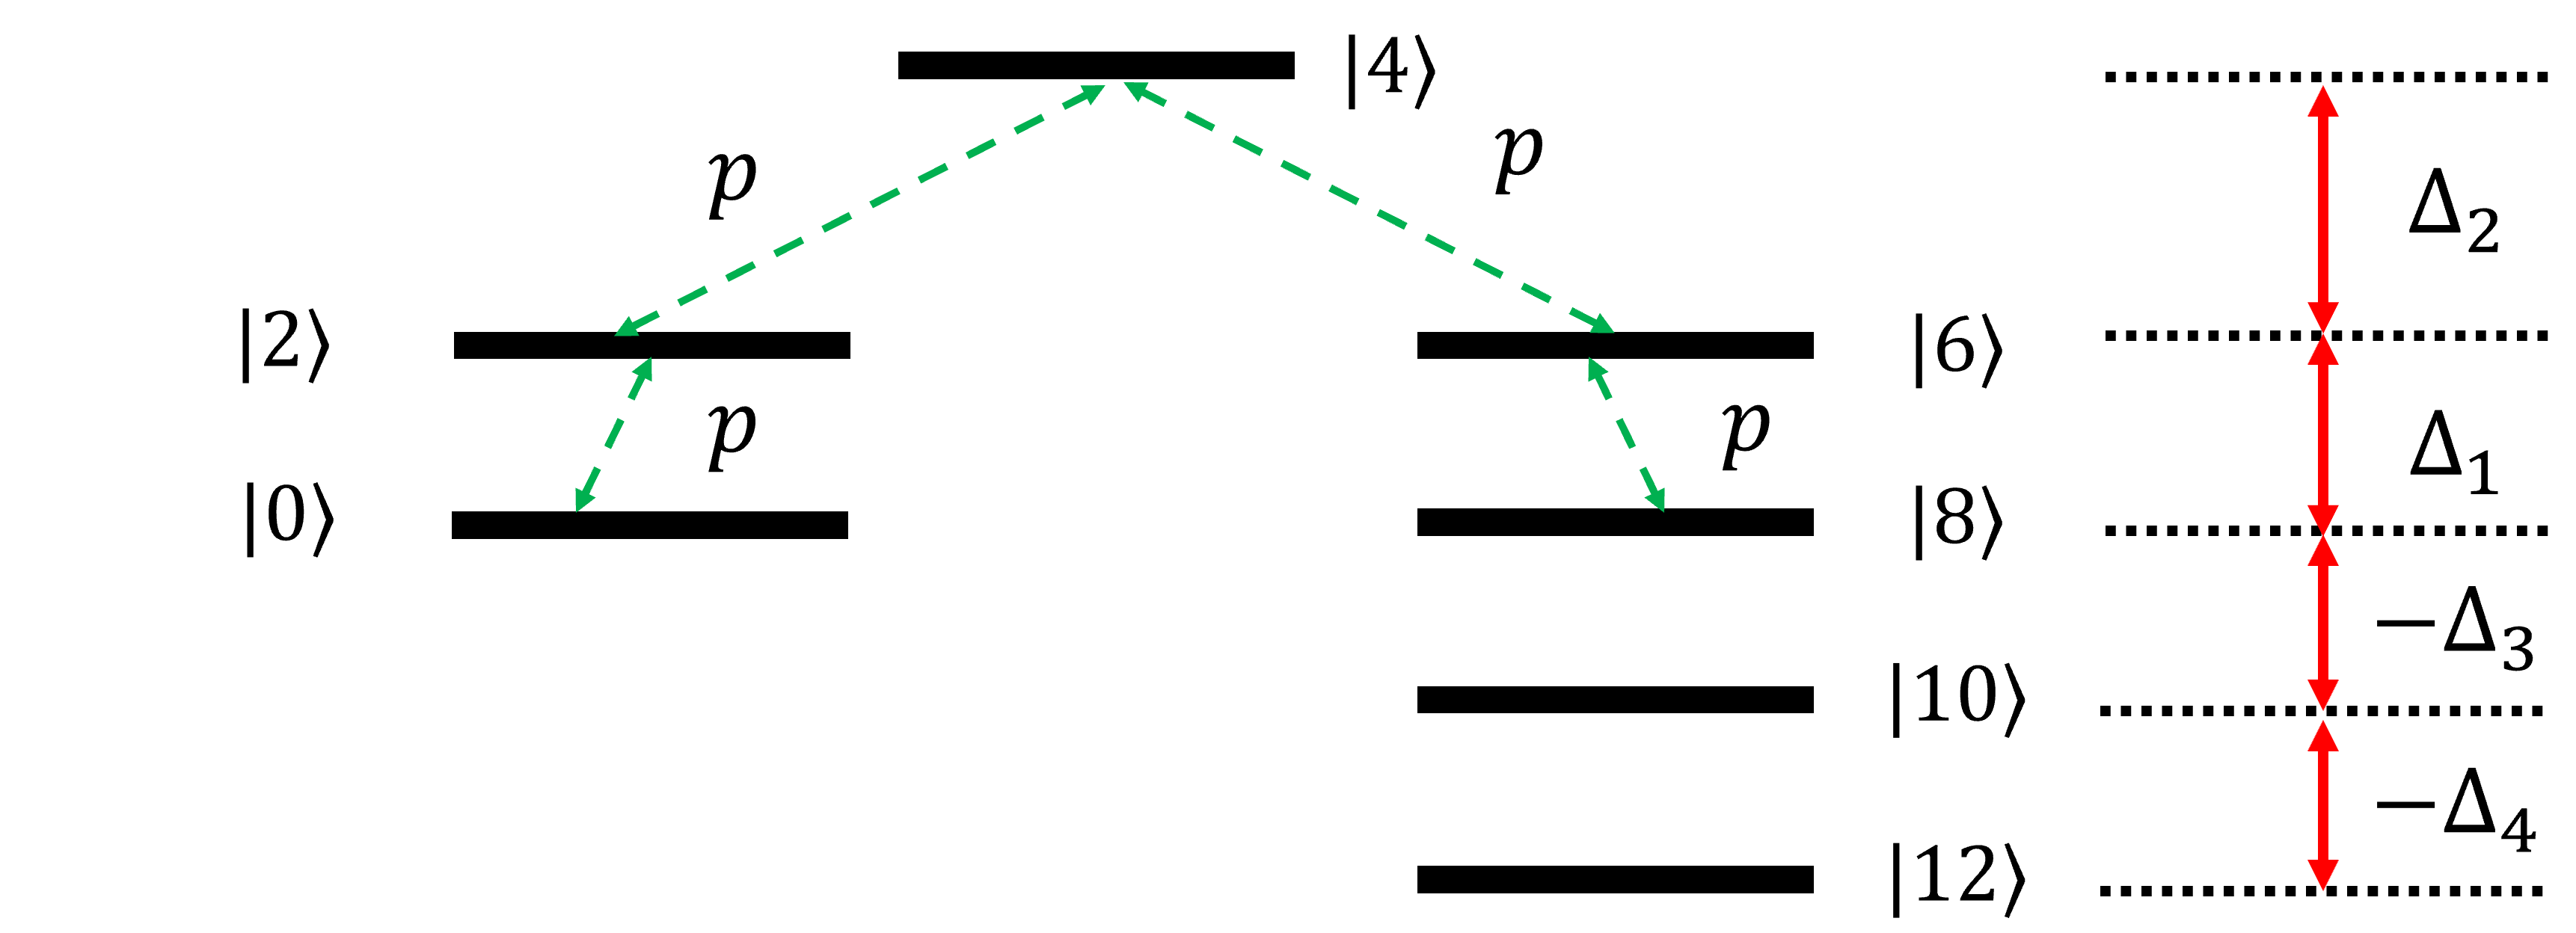
\includegraphics[width=10cm]{file/fig/effective_0and8/KPO_effective_0and8.png} \\
% \caption{有効模型の概念図}
% \label{fig:kpo_effective_0and8}
% \end{figure}

\begin{align}
     \hat{H}_{\rm{KPO}}^{\rm{eff}}&=
   \bordermatrix{     
    & \bra{0} &  \bra{2} &  \bra{4}&  \bra{6}&  \bra{8} &\bra{10} &\bra{12}\cr
   \ket{0}&E_0&p_1&0&0&0&0&0\cr
  \ket{2}&p_1&E_2&p_2&0&0&0&0\cr
  \ket{4}&0&p_2&E_4&p_3&0&0&0\cr
  \ket{6}&0&0&p_3&E_6&p_4&0&0\cr
  \ket{8}&0&0&0&p_4&E_8&p_5&0\cr
  \ket{10}&0&0&0&0&p_5&E_{10}&p_6\cr
  \ket{12}&0&0&0&0&0&p_6&E_{12}\cr
            }
    %%%
    =
   \bordermatrix{     
    & \bra{0} &  \bra{2} &  \bra{4}&  \bra{6}&  \bra{8} &\bra{10} &\bra{12}\cr
   \ket{0}&0&p_1&0&0&0&0&0\cr
  \ket{2}&p_1&\Delta_1&p_2&0&0&0&0\cr
  \ket{4}&0&p_2&\Delta_2&p_3&0&0&0\cr
  \ket{6}&0&0&p_3&\Delta_1&p_4&0&0\cr
  \ket{8}&0&0&0&p_4&0&p_5&0\cr
  \ket{10}&0&0&0&0&p_5&-\Delta_3&p_6\cr
  \ket{12}&0&0&0&0&0&p_6&-\Delta_4\cr
            }\nn[10pt]
    %%%%%%%%%%%%%%%%%%%
    &=\hat{H}_0 + \hat{V} 
\end{align}
ここで,この有効模型の非摂動Hamiltonian $\hat{H}_0^{\rm{eff}}$と摂動Hamiltonian $\hat{V}^{\rm{eff}}$はそれぞれ以下のように与える:
\begin{align}
    \hat{H}_0^{\rm{eff}}&=\bordermatrix{
    & \bra{0} &  \bra{2} &  \bra{4}&  \bra{6}&  \bra{8} &\bra{10} &\bra{12}\cr
   \ket{0}&0&0&0&0&0&0&0\cr
  \ket{2}&0&\Delta_1&0&0&0&0&0\cr
  \ket{4}&0&0&\Delta_2&0&0&0&0\cr
  \ket{6}&0&0&0&\Delta_1&0&0&0\cr
  \ket{8}&0&0&0&0&0&0&0\cr
  \ket{10}&0&0&0&0&0&-\Delta_3&0\cr
  \ket{12}&0&0&0&0&0&0&-\Delta_4\cr}\nn[10pt]
  %%%%%%%%%%%%%%
  %%%%%%%%%%%%%%
  \hat{V}^{\rm{eff}}&=
   \bordermatrix{     
    & \bra{0} &  \bra{2} &  \bra{4}&  \bra{6}&  \bra{8} &\bra{10} &\bra{12}\cr
   \ket{0}&0&p_1&0&0&0&0&0\cr
  \ket{2}&p_1&0&p_2&0&0&0&0\cr
  \ket{4}&0&p_2&0&p_3&0&0&0\cr
  \ket{6}&0&0&p_3&0&p_4&0&0\cr
  \ket{8}&0&0&0&p_4&0&p_5&0\cr
  \ket{10}&0&0&0&0&p_5&0&p_6\cr
  \ket{12}&0&0&0&0&0&p_6&0\cr}\\[10pt]
    &=
   \bordermatrix{     
    & \bra{0} &  \bra{2} &  \bra{4}&  \bra{6}&  \bra{8} &\bra{10} &\bra{12}\cr
   \ket{0}&0&\sqrt{2\cdot1}p&0&0&0&0&0\cr
  \ket{2}&\sqrt{2\cdot1}p&0&\sqrt{4\cdot3}p&0&0&0&0\cr
  \ket{4}&0&\sqrt{4\cdot3}p&0&\sqrt{6\cdot5}p&0&0&0\cr
  \ket{6}&0&0&\sqrt{6\cdot5}p&0&\sqrt{8\cdot7}p&0&0\cr
  \ket{8}&0&0&0&\sqrt{8\cdot7}p&0&\sqrt{10\cdot9}p&0\cr
  \ket{10}&0&0&0&0&\sqrt{10\cdot9}p&0&\sqrt{12\cdot11}p\cr
  \ket{12}&0&0&0&0&0&\sqrt{12\cdot11}p&0\cr
            }
\end{align}
ここで,$p_1=\sqrt{2\cdot1}p$, $p_2=\sqrt{4\cdot3}p$, $p_3=\sqrt{6\cdot5}p$, $p_4=\sqrt{8\cdot7}p$, $p_5=\sqrt{10\cdot9}p$, $p_6=\sqrt{12\cdot11}p$である.


\subsection{}
次に,この有効模型の非摂動Hamiltonian $\hat{H}_0^{\rm{eff}}$に注目する.このHamiltonian $\hat{H}_0^{\rm{eff}}$はBlock対角化されており,$\{\ket{0}, \ket{2}, \ket{4}, \ket{6}, \ket{8}\}$と$\ket{10}, \ket{12}$で張られる部分空間に分けることができ, Hamiltonianは以下のように書き直すことができる:
\begin{equation}
    \hat{H}_0^{\rm{eff}}
    =\hat{H}_0^{0\to8} \bigoplus \hat{H}_0^{10,12}
\end{equation}
ここで,
    
\begin{align}
    \hat{H}_0^{0\to8}&=\bordermatrix{
    & \bra{0} &  \bra{2} &  \bra{4}&  \bra{6}&  \bra{8}\cr
   \ket{0}&0&p&0&0&0\cr
  \ket{2}&p&\Delta_1&p&0&0\cr
  \ket{4}&0&p&\Delta_2&p&0\cr
  \ket{6}&0&0&p&\Delta_1&p\cr
  \ket{8}&0&0&0&p&0\cr
  }\\[10pt]
  %%%%%%%%%%%%%%
  %%%%%%%%%%%%%%
  \hat{H}_0^{10,12}&=
   \bordermatrix{     
    & \bra{10} &\bra{12}\cr
   \ket{10}&-\Delta_3&0\cr
  \ket{12}&0&-\Delta_4\cr}
\end{align}
である.Hamiltonian $\hat{H}_0^{0\to8}$を対角化する.
% \begin{figure}[h]
% \centering
% 		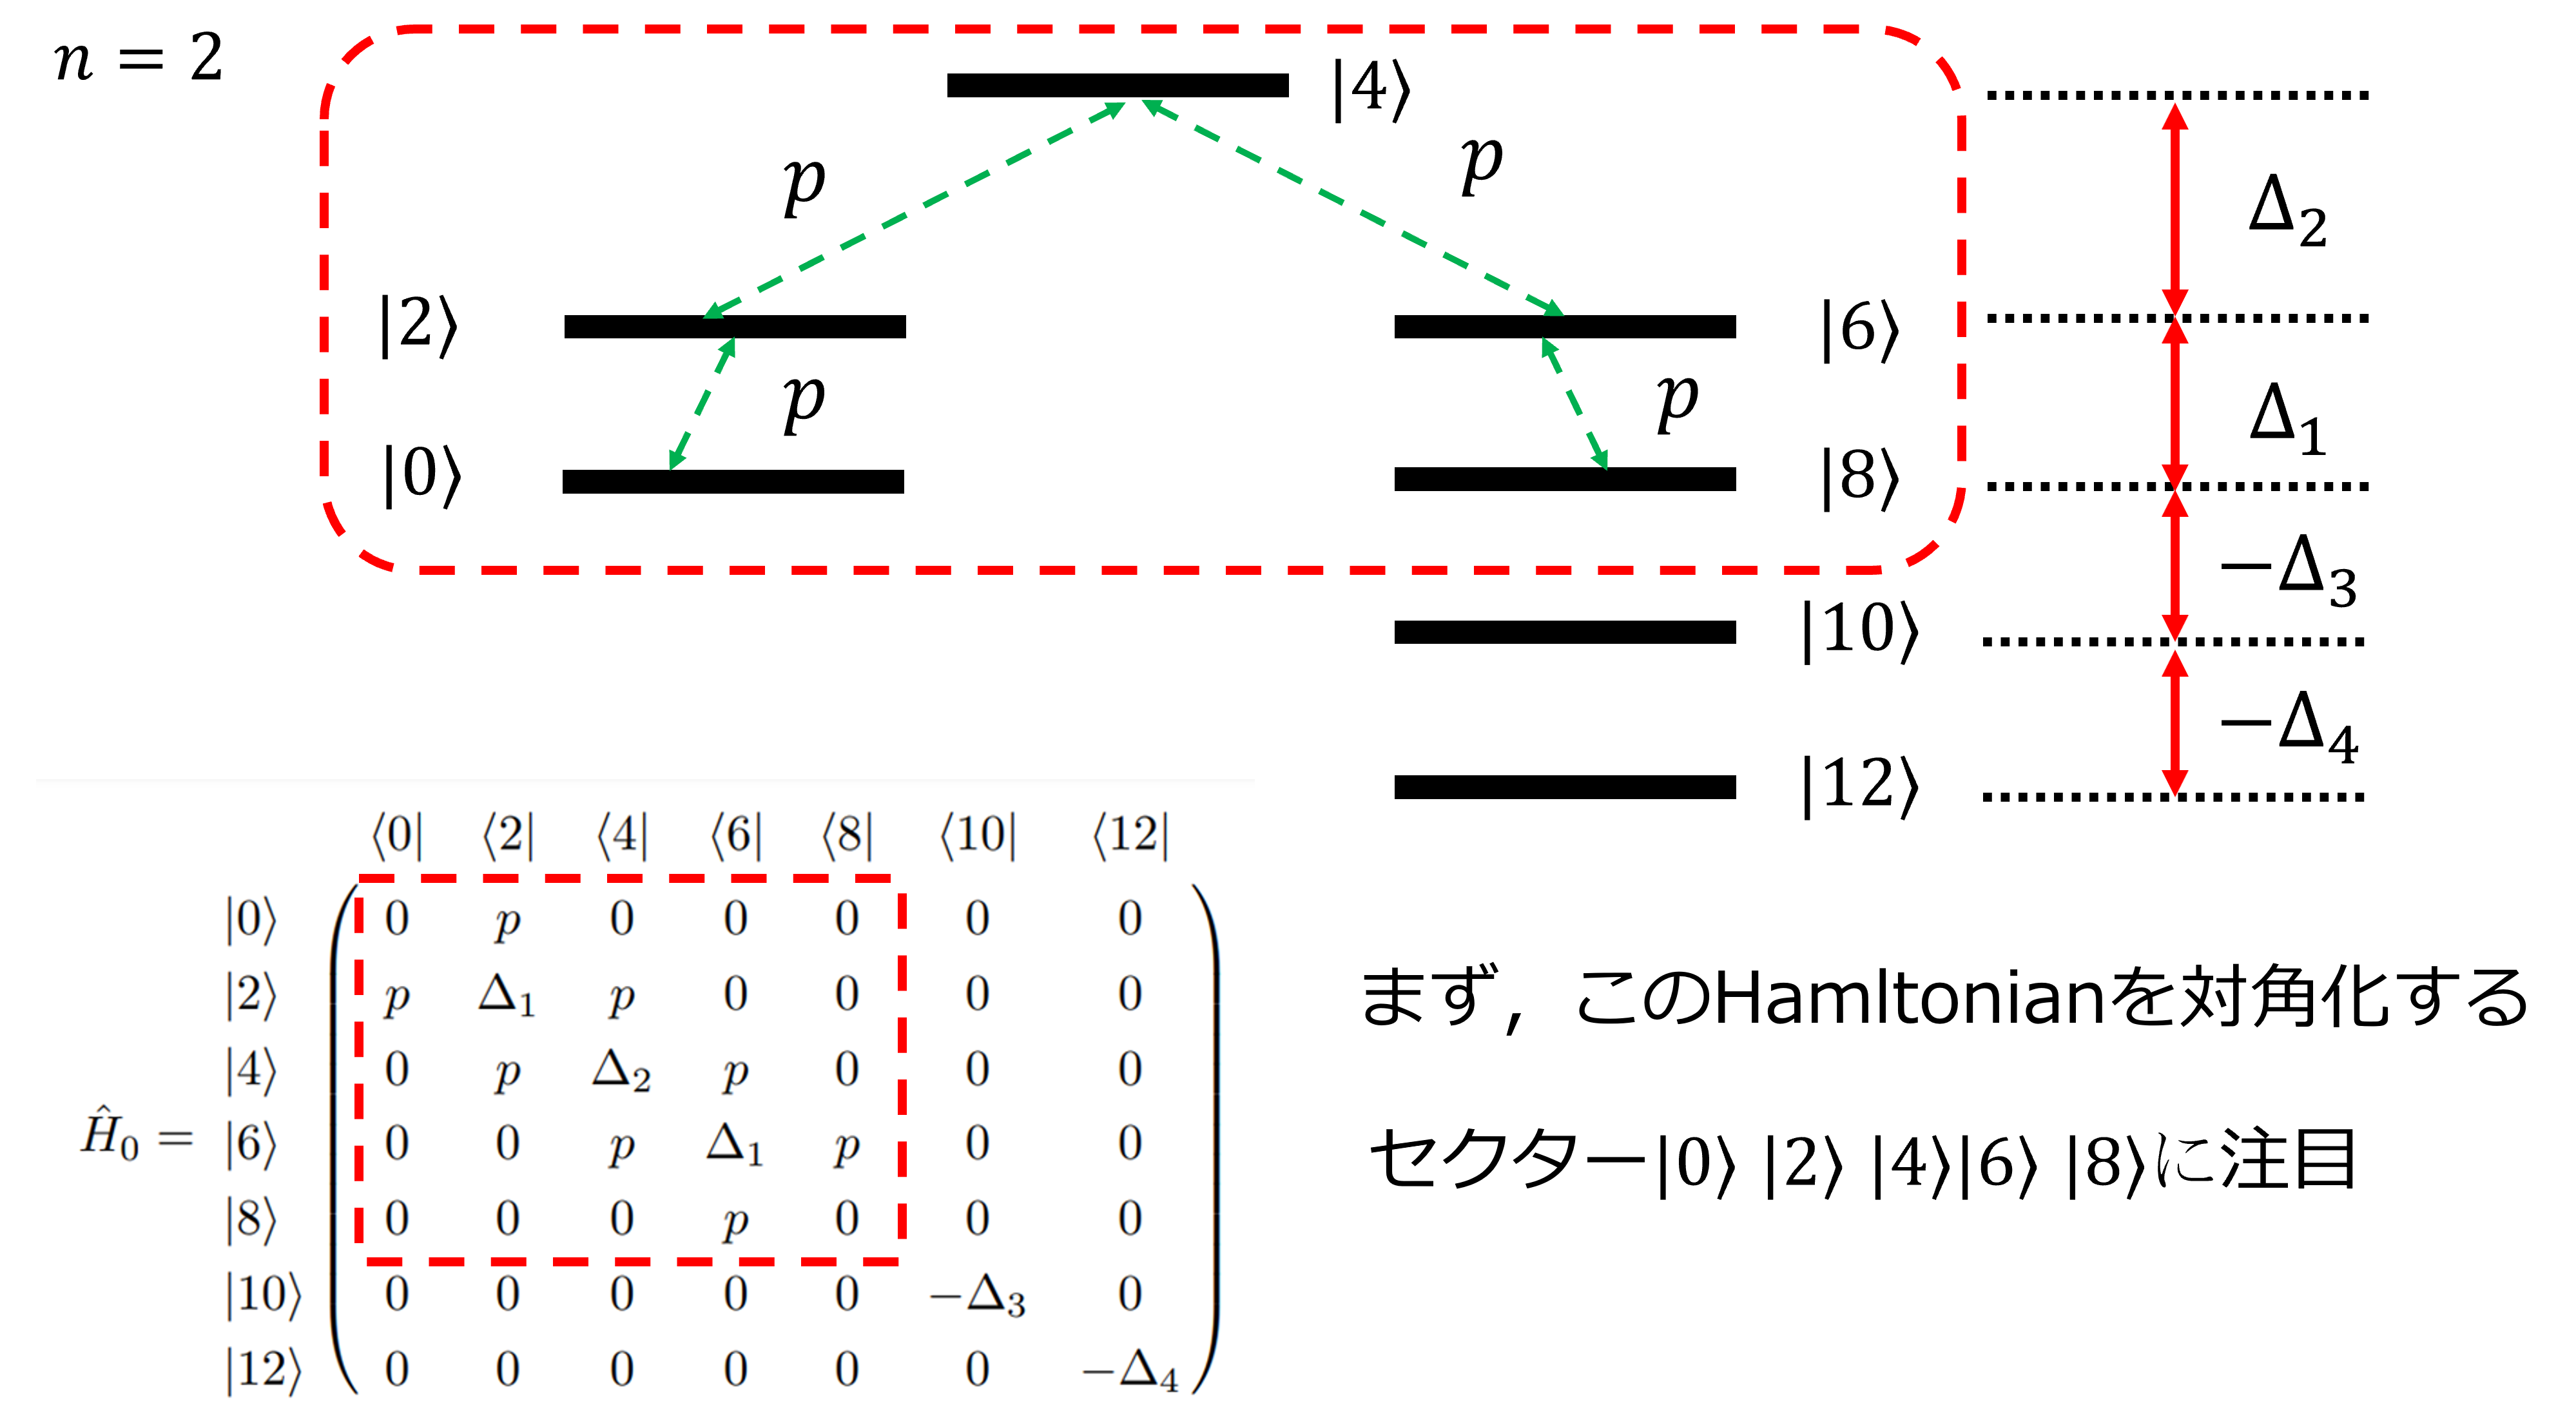
\includegraphics[width=10cm]{file/fig/effective_0and8/KPO_effective_0and8_1.png} \\
% \caption{有効模型の概念図}
% \label{fig:kpo_effective_0and8_1}
% \end{figure}
これを実行するために,まず,$\{\ket{2}, \ket{4}, \ket{6}\}$で張られる部分空間を考え,その空間におけるHamiltonian $\hat{H}^{2,4,6}$を以下のように定義する:
\begin{align}
    \hat{H}^{2,4,6}&=\bordermatrix{
    & \bra{2} &  \bra{4}&  \bra{6}\cr
  \ket{2}&\Delta_1&p_2&0\cr
  \ket{4}&p_2&\Delta_2&p_3\cr
  \ket{6}&0&p_3&\Delta_1\cr
  }
\end{align}
ここで,$\Delta_1>\Delta_2$を仮定する.このHamiltonianを対角化し,エネルギー固有値とエネルギー固有状態を求めると以下のように得られる:
%\section*{\textcolor{red}{Step1 : $n=2,4,6$の部分空間での厳密解}}


エネルギー固有値
\begin{align}
    E_{D_{2,6}}&=
    {\Delta_{1}}\\[10pt]
    %
    E_4&=
    \frac{1}{2}\left({\Delta_{1}}+{\Delta_{2}}-\sqrt{{\Delta_{1}}^2-2{\Delta_{1}}{\Delta_{2}}+{\Delta_{2}}^2+4p_2^2+4p_3^2}\right)\nn[10pt]
    &=\frac{1}{2}\left({\Delta_{1}}+{\Delta_{2}}-\sqrt{{
    (\Delta_{1}}-{\Delta_{2}})^2+4p_2^2+4p_3^2}\right)\\[10pt]
    %%
    E_{B_{2,6}}=&\frac{1}{2}\left({\Delta_{1}}+{\Delta_{2}}+\sqrt{{\Delta_{1}}^2-2{\Delta_{1}}{\Delta_{2}}+{\Delta_{2}}^2+4p_2^2+4p_3^2}\right)
    \nn[10pt]
    &=\frac{1}{2}\left({\Delta_{1}}+{\Delta_{2}}
    +\sqrt{{
    (\Delta_{1}}-{\Delta_{2}})^2+4p_2^2+4p_3^2}\right)
\end{align}
$p_2<p_3$とすると,$E_4< E_{B_{2,6}} < E_{D_{2,6}}$である.

固有状態$\ket{2}, \ket{4}, \ket{6}$で展開する.
\begin{align}
    \ket{\psi_D}&=C_0\left\{-\frac{{p_{3}}}{{p_{2}}},0,1\right\}\\[10pt]
    \ket{\psi_4}&=C_1\left\{\frac{{p_{2}}}{{p_{3}}},-\frac{{\Delta_{1}}-{\Delta_{2}}+\sqrt{{\Delta_{1}}^2-2{\Delta_{1}}{\Delta_{2}}+{\Delta_{2}}^2+4p_2^2+4p_3^2}}{2{p_{3}}},1\right\}\nn[10pt]
    &=C_1\left\{\frac{{p_{2}}}{{p_{3}}},-\frac{{\Delta_{1}}-{\Delta_{2}}
    +\sqrt{({\Delta_{1}}-{\Delta_{2}})^2+4p_2^2+4p_3^2}}{2{p_{3}}},1\right\}\nn[10pt]
    &=C_1\left\{\frac{{p_{2}}}{{p_{3}}},
    \epsilon_+({\Delta_{1}},{\Delta_{2}},
    p_2,p_3)
    ,1\right\}\\[10pt]
    %
    %
    \ket{\psi_{B_{2,6}}}&=C_2\left\{\frac{{p_{2}}}{{p_{3}}},-\frac{{\Delta_{1}}-{\Delta_{2}}-\sqrt{{\Delta_{1}}^2-2{\Delta_{1}}{\Delta_{2}}+{\Delta_{2}}^2+4p_2^2+4p_3^2}}{2{p_{3}}},1\right\}\nn[10pt]
    &=C_2\left\{\frac{{p_{2}}}{{p_{3}}},
    \epsilon_-({\Delta_{1}},{\Delta_{2}},p_2,p_3)
    ,1\right\}
\end{align}

\begin{align}
    \epsilon_{\textcolor{red}{\pm}}({\Delta_{1}},{\Delta_{2}},
    p_2,p_3)
    =-\frac{{\Delta_{1}}-{\Delta_{2}}
    \textcolor{red}{\pm}\sqrt{({\Delta_{1}}-{\Delta_{2}})^2+4p_2^2+4p_3^2}}{2{p_{3}}}
\end{align}


規格化
\begin{equation}
        \ket{D_{2,6}}\equiv\ket{\psi_0}
        =\left(
        \begin{array}{c}
       -\frac{{p_3}}{{p_2}\sqrt{\left|\frac{{p_3}}{{p_2}}\right|^2+1}}\\[20pt]
       0\\[10pt]
       \frac{1}{\sqrt{\left|\frac{{p_3}}{{p_2}}\right|^2+1}}\\[10pt]
        \end{array}
        \right)
        =\left(
        \begin{array}{c}
       -\frac{{p_3}}{\sqrt{\left|{{p_3}}\right|^2+\left|{{p_2}}\right|^2}}\\[20pt]
       0\\[10pt]
       \frac{{p_2}}{\sqrt{\left|{{p_3}}\right|^2+\left|{{p_2}}\right|^2}}\\[10pt]
        \end{array}
        \right)
\end{equation}

\begin{equation}
     \ket{4}\equiv\ket{\psi_1}=\left(
        \begin{array}{c}
       \frac{{p_2}}{{p_3}\sqrt{
       |\epsilon_{+}|^2
       +\left|\frac{{p_2}}{{p_3}}\right|^2+1}}\\[20pt]
       %
       %
       -\frac{{\Delta_1}-{\Delta_2}+\sqrt{{\Delta_1}^2-2{\Delta_1}{\Delta_2}+{\Delta_2}^2+4{p_2}^2+4{p_3}^2}}{2{p_3}\sqrt{
       |\epsilon_{+}|^2
       +\left|\frac{{p_2}}{{p_3}}\right|^2+1}}\\[20pt]
       %
       %
       \frac{1}{\sqrt{
       |\epsilon_{+}|^2
       +\left|\frac{{p_2}}{{p_3}}\right|^2+1}}
        \end{array}
        \right)
        %%%%%%%%%%%%%%%%%%%%%%%%%%%%
        %%%%%%%%%%%%%%%%%%%%%%%%%%%%
        =\left(
        \begin{array}{c}
       \frac{{p_2}}{{p_3}\sqrt{
       |\epsilon_{+}|^2
       +\left|\frac{{p_2}}{{p_3}}\right|^2+1}}\\[20pt]
       %
       %
       \frac{\epsilon_+}{
       \sqrt{
       |\epsilon_{+}|^2
       +\left|\frac{{p_2}}{{p_3}}\right|^2+1}}\\[20pt]
       %
       %
       \frac{1}{\sqrt{
       |\epsilon_{+}|^2
       +\left|\frac{{p_2}}{{p_3}}\right|^2+1}}
        \end{array}
        \right)
\end{equation}

\begin{equation}
     \ket{B_{2,6}}\equiv\ket{\psi_2}=\left(
        \begin{array}{c}
       \frac{{p_2}}{{p_3}\sqrt{
       |\epsilon_{-}|^2
       +\left|\frac{{p_2}}{{p_3}}\right|^2+1}}\\[20pt]
       %
       %
       -\frac{{\Delta_1}-{\Delta_2}-\sqrt{{\Delta_1}^2-2{\Delta_1}{\Delta_2}+{\Delta_2}^2+4{p_2}^2+4{p_3}^2}}{2{p_3}\sqrt{
       |\epsilon_{-}|^2
       +\left|\frac{{p_2}}{{p_3}}\right|^2+1}}\\[20pt]
       %
       %
       \frac{1}{\sqrt{
       |\epsilon_{-}|^2
       +\left|\frac{{p_2}}{{p_3}}\right|^2+1}}\\[10pt]
        \end{array}
        \right)
    %%%%%%%%%%%%%%%%%%%%%%%%%%%
    %%%%%%%%%%%%%%%%%%%%%%%%%%
    =\left(
        \begin{array}{c}
       \frac{{p_2}}{{p_3}\sqrt{
       |\epsilon_{-}|^2
       +\left|\frac{{p_2}}{{p_3}}\right|^2+1}}\\[20pt]
       %
       %
       \frac{
       \epsilon_-
       }{\sqrt{
       |\epsilon_{-}|^2
       +\left|\frac{{p_2}}{{p_3}}\right|^2+1}}\\[20pt]
       %
       %
       \frac{1}{\sqrt{
       |\epsilon_{-}|^2
       +\left|\frac{{p_1}}{{p_3}}\right|^2+1}}\\[10pt]
        \end{array}
        \right)
\end{equation}

ここで,パラメトリックドライブの振幅$\beta$が十分小さい場合,
次の状態を定義する:
\begin{align}
    \ket{D_{2,6}} &= -a_{D,2}\ket{2}+a_{D,6}\ket{6}\\[10pt]
    \ket{B_{2,6}} &= a_{B,2}\ket{2}+a_{B,6}\ket{6}
\end{align}
ここで,$a_{D,2} < a_{D,6}$, $a_{B,2} < a_{B,6}$である.

$1/\sqrt{2} \simeq 0.70710678118$

\begin{align}
    \hat{H}_0 &= E_{0}\ket{0}\bra{0} + E_8 \ket{8}\bra{8} + E_{D_{2,6}} \ket{D_{2,6}}\bra{D_{2,6}}+ E_{B_{2,6}} \ket{B_{2,6}}\bra{B_{2,6}}\\[10pt]
    \hat{V}&= \sqrt{2\cdot1}\beta\ket{0}\bra{2} + \sqrt{8\cdot7}\beta\ket{8}\bra{6} + {\rm{h.c.}}
\end{align}


\begin{align}
     \hat{H}_{\rm{KPO}}
    &=
   \bordermatrix{     
    & \bra{0} &  \bra{2} &  \bra{6}&  \bra{8}\cr
   \ket{0}&0&\sqrt{2\cdot1}\beta&0&0\cr
  \ket{2}&\sqrt{2\cdot1}\beta&\Delta_1&0&0\cr
  \ket{6}&0&0&\Delta_1&\sqrt{8\cdot7}\beta\cr
  \ket{8}&0&0&\sqrt{8\cdot7}\beta&0\cr
            }
\end{align}
次の状態を定義する:
\begin{align}
    \ket{D} &= \frac{1}{\sqrt{2}}(-\ket{2}+\ket{6})\\[10pt]
    \ket{B_{2,6}} &= \frac{1}{\sqrt{2}}(\ket{2}+\ket{6})
\end{align}




% \begin{align}
%      \hat{V}
%     &=
%    \bordermatrix{     
%     & \bra{0} &  \bra{8} &  \bra{D}&  \bra{B}\cr
%    \ket{0}&\langle{0|\hat{V}|0}\rangle&\langle{0|\hat{V}|8}\rangle&\langle{0|\hat{V}|D}\rangle
%    &\langle{0|\hat{V}|B}\rangle\cr
%   \ket{8}&\langle{8|\hat{V}|0}\rangle&\langle{8|\hat{V}|8}\rangle&\langle{8|\hat{V}|D}\rangle
%    &\langle{8|\hat{V}|B}\rangle\cr
%   \ket{D}&\langle{D|\hat{V}|0}\rangle&\langle{D|\hat{V}|8}\rangle&\langle{D|\hat{V}|D}\rangle
%    &\langle{D|\hat{V}|B}\rangle\cr
%   \ket{B_{2,6}}&\langle{B|\hat{V}|0}\rangle&\langle{B|\hat{V}|8}\rangle&\langle{B|\hat{V}|D}\rangle
%    &\langle{B|\hat{V}|B}\rangle\cr
%     }
% \end{align}



\subsection{}
部分空間$\{\ket{2}, \ket{4}, \ket{6}\}$内で,対角化することができたため,これで,$\ket{2}$と$\ket{6}$の縮退を解くことができた.したがって,次に,Hamiltonian $\hat{H}_0^{0\to8}$に対して,縮退する摂動論を適用し,そのエネルギー固有値と対応するエネルギー固有状態を求めていくことにする.
% \begin{figure}[h]
% \centering
% 		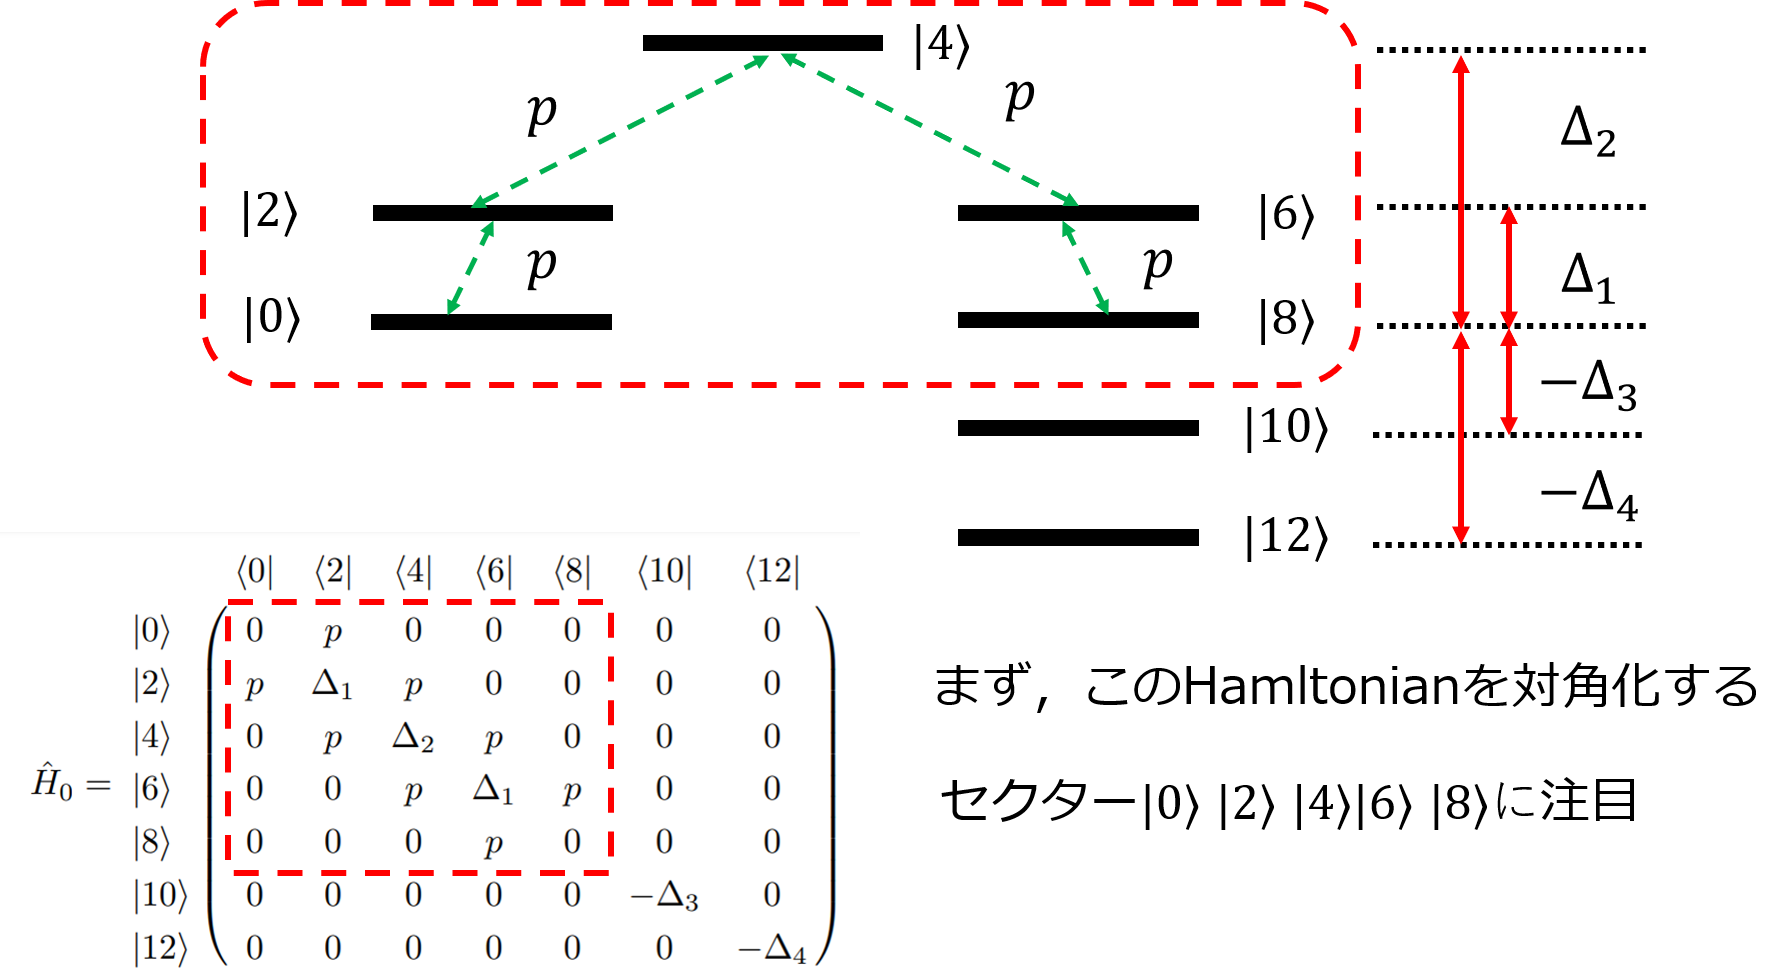
\includegraphics[width=10cm]{file/fig/effective_0and8/KPO_effective_0and8_2.png} \\
% \caption{有効模型の概念図}
% \label{fig:kpo_effective_0and8}
% \end{figure}


% \begin{figure}[h]
% \centering
% 		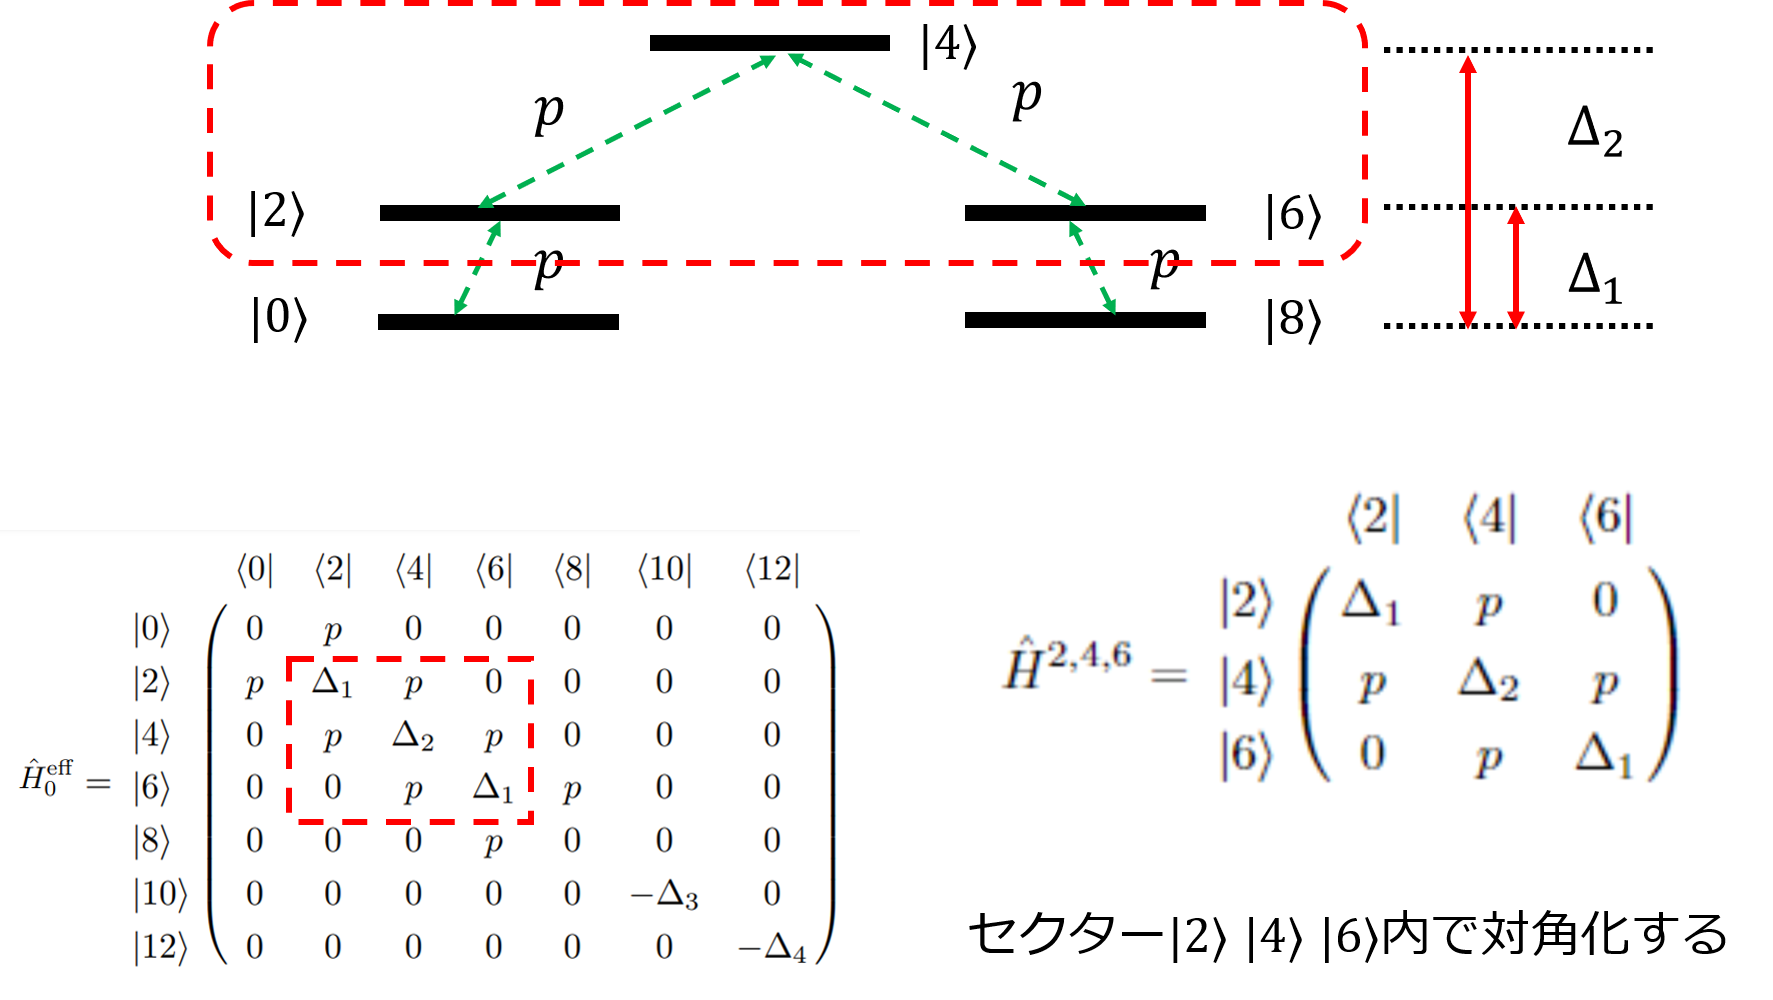
\includegraphics[width=10cm]{file/fig/effective_0and8/KPO_effective_0and8_3.png} \\
% \caption{有効模型の概念図}
% \label{fig:kpo_effective_0and8}
% \end{figure}


そのために,まず,摂動Hamiltonianを基底$\{\ket{D_{2,6}},\ket{B_{2,6}},\ket{0},\ket{8},\ket{10},\ket{12}\}$で展開する:
\begin{align}
  \hat{V}^{\rm{eff}}&=
   \bordermatrix{     
    & \bra{0} &  \bra{2} &  \bra{4}&  \bra{6}&  \bra{8} &\bra{10} &\bra{12}\cr
   \ket{0}&0&p_1&0&0&0&0&0\cr
  \ket{2}&p_1&0&0&0&0&0&0\cr
  \ket{4}&0&0&0&0&0&0&0\cr
  \ket{6}&0&0&0&0&p_4&0&0\cr
  \ket{8}&0&0&0&p_4&0&p_5&0\cr
  \ket{10}&0&0&0&0&p_5&0&p_6\cr
  \ket{12}&0&0&0&0&0&p_6&0\cr}
\end{align}

\begin{align}
  \hat{V}^{\rm{eff}}&=
    p_1\ket{0}\bra{2} + p_4\ket{8}\bra{6}
    + p_5\ket{10}\bra{8}
    + p_6\ket{12}\bra{10}+ {\rm{h.c.}}
\end{align}



\begin{align}
     \hat{V}^{\rm{eff}}&=\bordermatrix{
    & \bra{D_{2,6}}&  \bra{B_{2,6}} &\bra{0} &  \bra{8} &  \bra{10} &\bra{12}\cr
    %%
   \ket{D_{2,6}}&\langle{D_{2,6}|\hat{V}|D_{2,6}}\rangle&\langle{D_{2,6}|\hat{V}|B_{2,6}}\rangle
   &\langle{D_{2,6}|\hat{V}|0}\rangle&\langle{D_{2,6}|\hat{V}|8}\rangle
   &\langle{D_{2,6}|\hat{V}|10}\rangle&\langle{D_{2,6}|\hat{V}|12}\rangle\cr
   %
\ket{B_{2,6}}&\langle{B_{2,6}|\hat{V}|B_{2,6}}\rangle&\langle{B_{2,6}|\hat{V}|B_{2,6}}\rangle
   &\langle{B_{2,6}|\hat{V}|0}\rangle&\langle{B_{2,6}|\hat{V}|8}\rangle
   &\langle{B_{2,6}|\hat{V}|10}\rangle&\langle{B_{2,6}|\hat{V}|12}\rangle\cr
  %
  \ket{0}
  &\langle{0|\hat{V}|D_{2,6}}\rangle&\langle{0|\hat{V}|B_{2,6}}\rangle
  &\langle{0|\hat{V}|0}\rangle&\langle{0|\hat{V}|8}\rangle
  &\langle{0|\hat{V}|10}\rangle&\langle{0|\hat{V}|12}\rangle\cr
  %
  \ket{8}
  &\langle{8|\hat{V}|D_{2,6}}\rangle&\langle{8|\hat{V}|B_{2,6}}\rangle
  &\langle{8|\hat{V}|0}\rangle&\langle{8|\hat{V}|8}\rangle
   &\langle{8|\hat{V}|10}\rangle
   &\langle{8|\hat{V}|12}\rangle\cr
  %
  \ket{10}&\langle{10|\hat{V}|D_{2,6}}\rangle&\langle{10|\hat{V}|B_{2,6}}\rangle
   &\langle{10|\hat{V}|0}\rangle&\langle{10|\hat{V}|8}\rangle
   &\langle{10|\hat{V}|10}\rangle&\langle{10|\hat{V}|12}\rangle\cr
  %
  \ket{12}&\langle{12|\hat{V}|D_{2,6}}\rangle&\langle{12|\hat{V}|B_{2,6}}\rangle
   &\langle{12|\hat{V}|0}\rangle&\langle{12|\hat{V}|8}\rangle
   &\langle{12|\hat{V}|10}\rangle&\langle{12|\hat{V}|12}\rangle\cr}
   \nn[10pt]
   &=\bordermatrix{
    & \bra{D_{2,6}}&  \bra{B_{2,6}} &\bra{0} &  \bra{8} &  \bra{10} &\bra{12}\cr
    %%
   \ket{D_{2,6}}&0&0
   &\langle{D_{2,6}|\hat{V}|0}\rangle&\langle{D_{2,6}|\hat{V}|8}\rangle
   &0&0\cr
   %
\ket{B_{2,6}}&0&0
   &\langle{B_{2,6}|\hat{V}|0}\rangle&\langle{B_{2,6}|\hat{V}|8}\rangle
   &0&0\cr
  %
  \ket{0}
  &\langle{0|\hat{V}|D_{2,6}}\rangle&\langle{0|\hat{V}|B_{2,6}}\rangle
  &0&0
  &0&0\cr
  %
  \ket{8}
  &\langle{8|\hat{V}|D_{2,6}}\rangle&\langle{8|\hat{V}|B_{2,6}}\rangle
  &0&0
   &\langle{8|\hat{V}|10}\rangle
   &0\cr
  %
  \ket{10}&0&0
   &0&\langle{10|\hat{V}|8}\rangle
   &0&\langle{10|\hat{V}|12}\rangle\cr
  %
  \ket{12}&0&0
   &0&0
   &\langle{12|\hat{V}|10}\rangle&0\cr}
\end{align}


\begin{align}
     \hat{V}^{\rm{eff}}&=\bordermatrix{
    & \bra{D_{2,6}}&  \bra{B_{2,6}} &\bra{0} &  \bra{8} &  \bra{10} &\bra{12}\cr
    %%
   \ket{D_{2,6}}
   &0&0
   &-a_{D,2}p_1&a_{D,6}p_4
   &0&0\cr
   %
\ket{B_{2,6}}&0&0
   &a_{B,2}p_1&a_{B,6}p_4
   &0&0\cr
  %
  \ket{0}
  &-a_{D,2}p_1&a_{B,2}p_1
  &0&0
  &0&0\cr
  %
  \ket{8}
  &a_{D,6}p_4&a_{B,6}p_4
  &0&0
   &p_5
   &0\cr
  %
  \ket{10}&0&0
   &0&p_5
   &0&p_6\cr
  %
  \ket{12}&0&0
   &0&0
   &p_6&0
   \cr}
\end{align}

行列要素の計算は以下である:
\begin{align}
    \langle{D_{2,6}|\hat{V}^{\rm{eff}}|0}\rangle
    &=\langle{0|\hat{V}^{\rm{eff}}|D_{2,6}}\rangle
    =-a_{D,2}\braket{0|\hat{V}^{\rm{eff}}|2}+a_{D,6}\braket{0|\hat{V}^{\rm{eff}}|6}
    =-a_{D,2}p_1\\[10pt]
    %%%%%%
    \langle{D_{2,6}|\hat{V}^{\rm{eff}}|8}\rangle
    &=\langle{8|\hat{V}^{\rm{eff}}|D_{2,6}}\rangle
    =-a_{D,2}\braket{8|\hat{V}^{\rm{eff}}|2}+a_{D,6}\braket{8|\hat{V}^{\rm{eff}}|6}
    =a_{D,6}p_4\\[10pt]
    %%%%%%
    \langle{D_{2,6}|\hat{V}^{\rm{eff}}|10}\rangle
    &=\langle{10|\hat{V}^{\rm{eff}}|D_{2,6}}\rangle
    =0\\[10pt]
    %%%%%%
    \langle{D_{2,6}|\hat{V}^{\rm{eff}}|12}\rangle
    &=\langle{12|\hat{V}^{\rm{eff}}|D_{2,6}}\rangle
    =0
\end{align}


\begin{align}
    \langle{B_{2,6}|\hat{V}^{\rm{eff}}|0}\rangle
    &=\langle{0|\hat{V}^{\rm{eff}}|B_{2,6}}\rangle
    =a_{B,2}\braket{0|\hat{V}^{\rm{eff}}|2}+a_{B,6}\braket{0|\hat{V}^{\rm{eff}}|6}
    =a_{B,2}p_1\\[10pt]
    %%%%%%
    \langle{B_{2,6}|\hat{V}^{\rm{eff}}|8}\rangle
    &=\langle{8|\hat{V}^{\rm{eff}}|B_{2,6}}\rangle
    =a_{B,2}\braket{8|\hat{V}^{\rm{eff}}|2}+a_{B,6}\braket{8|\hat{V}^{\rm{eff}}|6}
    =a_{B,6}p_4\\[10pt]
    %%%%%%
    \langle{B_{2,6}|\hat{V}^{\rm{eff}}|10}\rangle
    &=\langle{10|\hat{V}^{\rm{eff}}|B_{2,6}}\rangle
    =0\\[10pt]
    %%%%%%
    \langle{B_{2,6}|\hat{V}^{\rm{eff}}|12}\rangle
    &=\langle{12|\hat{V}^{\rm{eff}}|B_{2,6}}\rangle
    =0
\end{align}
これら以外の行列要素は元の摂動Hamiltonianより明らかである.

\section*{\textcolor{red}{STEP1 : 固有状態の1次摂動を計算する}}
この摂動Hamiltonianに従って,縮退のある摂動論を適用していく.まず,固有状態の1次摂動を計算する:
\begin{align}
    \ket{\varphi_{n,0}^{(1)}}
    &=
    \sum_{\textcolor{red}{\gamma\neq0}}|\varphi^{(0)}_n;8\rangle\rangle
    \textcolor{red}{\frac{1}{(E^{(2)}_{n,0}-E^{(2)}_{n,8})}
    \sum_{m\neq n}\Biggl[\sum_{p\neq n}
    \frac{\langle\braket{\varphi^{(0)}_{n};\gamma|\hat{V}|\varphi^{(0)}_m}
    \langle{\varphi^{(0)}_{m}|\hat{V}|\varphi^{(0)}_p}\rangle
    \braket{\varphi^{(0)}_{p}|\hat{V}|\varphi^{(0)}_n;0}\rangle}
    {(\epsilon_n-\epsilon_m)(\epsilon_n-\epsilon_p)}}\nn[10pt]
    %
    &\hspace{100pt}
    \textcolor{red}{-E^{(1)}_n
    \frac{\langle\braket{\varphi^{(0)}_{n};\gamma|\hat{V}|\varphi^{(0)}_m}
    \braket{\varphi^{(0)}_{m}|\hat{V}|\varphi^{(0)}_n;0}\rangle}{(\epsilon_n-\epsilon_m)^2}
    \Biggr]}
    \nn[10pt]
    %
    &\hspace{200pt}+
    \sum_{m\neq n}\ket{\varphi^{(0)}_m}
    \textcolor{blue}{
    \frac{\braket{\varphi^{(0)}_{m}|\hat{V}|\varphi^{(0)}_n;0}\rangle}{(\epsilon_n-\epsilon_m)}}\nn[10pt]
    %%%%%%%%%%%%%%%%%%%%
    %%%%%%%%%%%%%%%%%%%%
    &=
    |\varphi^{(0)}_n;8\rangle\rangle
    \textcolor{red}{\frac{1}{(E^{(2)}_{n,0}-E^{(2)}_{n,8})}
    \sum_{m\neq n}\Biggl[\sum_{p\neq n}
    \frac{\langle\braket{\varphi^{(0)}_{n};8|\hat{V}|\varphi^{(0)}_m}
    \langle{\varphi^{(0)}_{m}|\hat{V}|\varphi^{(0)}_p}\rangle
    \braket{\varphi^{(0)}_{p}|\hat{V}|\varphi^{(0)}_n;0}\rangle}
    {(\epsilon_n-\epsilon_m)(\epsilon_n-\epsilon_p)}}\nn[10pt]
    %
    &\hspace{100pt}
    \textcolor{red}{-E^{(1)}_n
    \frac{\langle\braket{\varphi^{(0)}_{n};8|\hat{V}|\varphi^{(0)}_m}
    \braket{\varphi^{(0)}_{m}|\hat{V}|\varphi^{(0)}_n;0}\rangle}{(\epsilon_n-\epsilon_m)^2}
    \Biggr]}
    \nn[10pt]
    %
    &\hspace{200pt}+
    \sum_{m\neq n}\ket{\varphi^{(0)}_m}
    \textcolor{blue}{
    \frac{\braket{\varphi^{(0)}_{m}|\hat{V}|\varphi^{(0)}_n;0}\rangle}{(\epsilon_n-\epsilon_m)}}\nn[10pt]
    %%%%%%%%%%%%%%%%%%%%
    %%%%%%%%%%%%%%%%%%%%
    &=
    |\varphi^{(0)}_n;8\rangle\rangle
    \textcolor{red}{\frac{1}{(E^{(2)}_{n,0}-E^{(2)}_{n,8})}
    \sum_{m\neq n}\Biggl[
    \frac{\langle\braket{\varphi^{(0)}_{n};8|\hat{V}|\varphi^{(0)}_m}
    \langle{\varphi^{(0)}_{m}|\hat{V}|\varphi^{(0)}_{D_{2,6}}}\rangle
    \braket{\varphi^{(0)}_{D_{2,6}}|\hat{V}|\varphi^{(0)}_n;0}\rangle}
    {(\epsilon_n-\epsilon_m)(\epsilon_n-\epsilon_{D_{2,6}})}}\nn[10pt]
    %
    &\hspace{100pt}
    +{\frac{\langle\braket{\varphi^{(0)}_{n};8|\hat{V}|\varphi^{(0)}_m}
    \langle{\varphi^{(0)}_{m}|\hat{V}|\varphi^{(0)}_{B_{2,6}}}\rangle
    \braket{\varphi^{(0)}_{B_{2,6}}|\hat{V}|\varphi^{(0)}_n;0}\rangle}
    {(\epsilon_n-\epsilon_m)(\epsilon_n-\epsilon_{B_{2,6}})}}\nn[10pt]
    %
    &\hspace{100pt}
    +{\frac{\langle\braket{\varphi^{(0)}_{n};8|\hat{V}|\varphi^{(0)}_m}
    \langle{\varphi^{(0)}_{m}|\hat{V}|10}\rangle
    \braket{10|\hat{V}|\varphi^{(0)}_n;0}\rangle}
    {(\epsilon_n-\epsilon_m)(\epsilon_n-\epsilon_{10})}}\nn[10pt]
    %
    %
    &\hspace{100pt}
    \textcolor{red}{-E^{(1)}_n
    \frac{\langle\braket{\varphi^{(0)}_{n};8|\hat{V}|\varphi^{(0)}_m}
    \braket{\varphi^{(0)}_{m}|\hat{V}|\varphi^{(0)}_n;0}\rangle}{(\epsilon_n-\epsilon_m)^2}
    \Biggr]}
    \nn[10pt]
    %
    &\hspace{200pt}+
    \sum_{m\neq n}\ket{\varphi^{(0)}_m}
    \textcolor{blue}{
    \frac{\braket{\varphi^{(0)}_{m}|\hat{V}|\varphi^{(0)}_n;0}\rangle}{(\epsilon_n-\epsilon_m)}}
\end{align}



\begin{align}
    \ket{\varphi_{n,0}^{(1)}}
    &=
    |\varphi^{(0)}_n;8\rangle\rangle
    \textcolor{red}{\frac{1}{(E^{(2)}_{n,0}-E^{(2)}_{n,8})}}\nn[10pt]
    &\times
    \textcolor{red}{\Biggl[\Biggl\{
    \frac{\langle\braket{\varphi^{(0)}_{n};8|\hat{V}|\varphi^{(0)}_{D_{2,6}}}
    \langle{\varphi^{(0)}_{D_{2,6}}|\hat{V}|\varphi^{(0)}_{D_{2,6}}}\rangle
    \braket{\varphi^{(0)}_{D_{2,6}}|\hat{V}|\varphi^{(0)}_n;0}\rangle}
    {(\epsilon_n-\epsilon_{D_{2,6}})(\epsilon_n-\epsilon_{D_{2,6}})}}\nn[10pt]
    %
    &\hspace{100pt}
    +{\frac{\langle\braket{\varphi^{(0)}_{n};8|\hat{V}|\varphi^{(0)}_{D_{2,6}}}
    \langle{\varphi^{(0)}_{D_{2,6}}|\hat{V}|\varphi^{(0)}_{B_{2,6}}}\rangle
    \braket{\varphi^{(0)}_{B_{2,6}}|\hat{V}|\varphi^{(0)}_n;0}\rangle}
    {(\epsilon_n-\epsilon_{D_{2,6}})(\epsilon_n-\epsilon_{B_{2,6}})}}\nn[10pt]
    %
    %
    &\hspace{100pt}
    +{\frac{\langle\braket{\varphi^{(0)}_{n};8|\hat{V}|\varphi^{(0)}_{D_{2,6}}}
    \langle{\varphi^{(0)}_{{D_{2,6}}}|\hat{V}|\varphi^{(0)}_{10}}\rangle
    \braket{\varphi^{(0)}_{10}|\hat{V}|\varphi^{(0)}_n;0}\rangle}
    {(\epsilon_n-\epsilon_{D_{2,6}})(\epsilon_n-\epsilon_{10})}}\nn[10pt]
    %
    &\hspace{100pt}
    \textcolor{red}{-E^{(1)}_n
    \frac{\langle\braket{\varphi^{(0)}_{n};8|\hat{V}|\varphi^{(0)}_{D_{2,6}}}
    \braket{\varphi^{(0)}_{D_{2,6}}|\hat{V}|\varphi^{(0)}_n;0}\rangle}{(\epsilon_n-\epsilon_{D_{2,6}})^2}
    \Biggr\}}
    \nn[10pt]
    %
    %
    &+\textcolor{red}{\Biggl\{
    \frac{\langle\braket{\varphi^{(0)}_{n};8|\hat{V}|\varphi^{(0)}_{B_{2,6}}}
    \langle{\varphi^{(0)}_{B_{2,6}}|\hat{V}|\varphi^{(0)}_{D_{2,6}}}\rangle
    \braket{\varphi^{(0)}_{D_{2,6}}|\hat{V}|\varphi^{(0)}_n;0}\rangle}
    {(\epsilon_n-\epsilon_{B_{2,6}})(\epsilon_n-\epsilon_{D_{2,6}})}}\nn[10pt]
    %
    &\hspace{100pt}
    +{\frac{\langle\braket{\varphi^{(0)}_{n};8|\hat{V}|\varphi^{(0)}_{B_{2,6}}}
    \langle{\varphi^{(0)}_{B_{2,6}}|\hat{V}|\varphi^{(0)}_{B_{2,6}}}\rangle
    \braket{\varphi^{(0)}_{B_{2,6}}|\hat{V}|\varphi^{(0)}_n;0}\rangle}
    {(\epsilon_n-\epsilon_{B_{2,6}})(\epsilon_n-\epsilon_{B_{2,6}})}}\nn[10pt]
    %
    %
    &\hspace{100pt}
    +{\frac{\langle\braket{\varphi^{(0)}_{n};8|\hat{V}|\varphi^{(0)}_{B_{2,6}}}
    \langle{\varphi^{(0)}_{{B_{2,6}}}|\hat{V}|\varphi^{(0)}_{10}}\rangle
    \braket{\varphi^{(0)}_{10}|\hat{V}|\varphi^{(0)}_n;0}\rangle}
    {(\epsilon_n-\epsilon_{B_{2,6}})(\epsilon_n-\epsilon_{10})}}\nn[10pt]
    %
    &\hspace{100pt}
    \textcolor{red}{-E^{(1)}_n
    \frac{\langle\braket{\varphi^{(0)}_{n};8|\hat{V}|\varphi^{(0)}_{B_{2,6}}}
    \braket{\varphi^{(0)}_{B_{2,6}}|\hat{V}|\varphi^{(0)}_n;0}\rangle}{(\epsilon_n-\epsilon_{B_{2,6}})^2}
    \Biggr\}\Biggr]}
    \nn[10pt]
    %
    %
    &+\textcolor{red}{\Biggl\{
    \frac{\langle\braket{\varphi^{(0)}_{n};8|\hat{V}|\varphi^{(0)}_{10}}
    \langle{\varphi^{(0)}_{10}|\hat{V}|\varphi^{(0)}_{D_{2,6}}}\rangle
    \braket{\varphi^{(0)}_{D_{2,6}}|\hat{V}|\varphi^{(0)}_n;0}\rangle}
    {(\epsilon_n-\epsilon_{10})(\epsilon_n-\epsilon_{D_{2,6}})}}\nn[10pt]
    %
    &\hspace{100pt}
    +{\frac{\langle\braket{\varphi^{(0)}_{n};8|\hat{V}|\varphi^{(0)}_{10}}
    \langle{\varphi^{(0)}_{10}|\hat{V}|\varphi^{(0)}_{B_{2,6}}}\rangle
    \braket{\varphi^{(0)}_{B_{2,6}}|\hat{V}|\varphi^{(0)}_n;0}\rangle}
    {(\epsilon_n-\epsilon_{10})(\epsilon_n-\epsilon_{B_{2,6}})}}\nn[10pt]
    %
    %
    &\hspace{100pt}
    +{\frac{\langle\braket{\varphi^{(0)}_{n};8|\hat{V}|\varphi^{(0)}_{10}}
    \langle{\varphi^{(0)}_{{10}}|\hat{V}|\varphi^{(0)}_{10}}\rangle
    \braket{\varphi^{(0)}_{10}|\hat{V}|\varphi^{(0)}_n;0}\rangle}
    {(\epsilon_n-\epsilon_{10})(\epsilon_n-\epsilon_{10})}}\nn[10pt]
    %
    &\hspace{100pt}
    \textcolor{red}{-E^{(1)}_n
    \frac{\langle\braket{\varphi^{(0)}_{n};8|\hat{V}|\varphi^{(0)}_{10}}
    \braket{\varphi^{(0)}_{10}|\hat{V}|\varphi^{(0)}_n;0}\rangle}{(\epsilon_n-\epsilon_{10})^2}
    \Biggr\}\Biggr]}
    \nn[10pt]
    %
    %
    &+
    \ket{\varphi^{(0)}_{D_{2,6}}}
    \textcolor{blue}{
    \frac{\braket{\varphi^{(0)}_{D_{2,6}}|\hat{V}|\varphi^{(0)}_n;0}\rangle}{(\epsilon_n-\epsilon_{D_{2,6}})}}
    +
    \ket{\varphi^{(0)}_{B_{2,6}}}
    \textcolor{blue}{
    \frac{\braket{\varphi^{(0)}_{B_{2,6}}|\hat{V}|\varphi^{(0)}_n;0}\rangle}{(\epsilon_n-\epsilon_{B_{2,6}})}}
    +
    \ket{\varphi^{(0)}_{10}}
    \textcolor{blue}{
    \frac{\braket{\varphi^{(0)}_{10}|\hat{V}|\varphi^{(0)}_n;0}\rangle}{(\epsilon_n-\epsilon_{10})}}
\end{align}

$|\varphi^{(0)}_{n};0\rangle\rangle=C_{0,0}\ket{0}+C_{8,0}\ket{8}$, 
$|\varphi^{(0)}_{n};8\rangle\rangle=C_{0,8}\ket{0}+C_{8,8}\ket{8}$,  $|\varphi^{(0)}_{D_{2,6}}\rangle=\ket{D_{2,6}}$, $|\varphi^{(0)}_{B_{2,6}}\rangle=\ket{B_{2,6}}$, 
$|\varphi^{(0)}_{10}\rangle=\ket{10}$であるから,


\begin{align}
    \ket{\varphi_{n,0}^{(1)}}
    &=
    |\varphi^{(0)}_n;8\rangle\rangle
    \textcolor{red}{\frac{1}{(E^{(2)}_{n,0}-E^{(2)}_{n,8})}}\nn[10pt]
    &\times
    \textcolor{red}{\Biggl[\Biggl\{
    \frac{\langle\braket{\varphi^{(0)}_{n};8|\hat{V}|D_{2,6}}
    \langle{D_{2,6}|\hat{V}|D_{2,6}}\rangle
    \braket{D_{2,6}|\hat{V}|\varphi^{(0)}_n;0}\rangle}
    {(\epsilon_n-\epsilon_{D_{2,6}})(\epsilon_n-\epsilon_{D_{2,6}})}}\nn[10pt]
    %
    &\hspace{100pt}
    +{\frac{\langle\braket{\varphi^{(0)}_{n};8|\hat{V}|D_{2,6}}
    \langle{D_{2,6}|\hat{V}|B_{2,6}}\rangle
    \braket{B_{2,6}|\hat{V}|\varphi^{(0)}_n;0}\rangle}
    {(\epsilon_n-\epsilon_{D_{2,6}})(\epsilon_n-\epsilon_{B_{2,6}})}}\nn[10pt]
    %
    %
    &\hspace{100pt}
    +{\frac{\langle\braket{\varphi^{(0)}_{n};8|\hat{V}|D_{2,6}}
    \langle{D_{2,6}|\hat{V}|10}\rangle
    \braket{10|\hat{V}|\varphi^{(0)}_n;0}\rangle}
    {(\epsilon_n-\epsilon_{D_{2,6}})(\epsilon_n-\epsilon_{10})}}\nn[10pt]
    %
    &\hspace{100pt}
    \textcolor{red}{-E^{(1)}_n
    \frac{\langle\braket{\varphi^{(0)}_{n};8|\hat{V}|D_{2,6}}
    \braket{D_{2,6}|\hat{V}|\varphi^{(0)}_n;0}\rangle}{(\epsilon_n-\epsilon_{D_{2,6}})^2}
    \Biggr\}}
    \nn[10pt]
    %
    %
    &+\textcolor{red}{\Biggl\{
    \frac{\langle\braket{\varphi^{(0)}_{n};8|\hat{V}|B_{2,6}}
    \langle{B_{2,6}|\hat{V}|D_{2,6}}\rangle
    \braket{D_{2,6}|\hat{V}|\varphi^{(0)}_n;0}\rangle}
    {(\epsilon_n-\epsilon_{B_{2,6}})(\epsilon_n-\epsilon_{D_{2,6}})}}\nn[10pt]
    %
    &\hspace{100pt}
    +{\frac{\langle\braket{\varphi^{(0)}_{n};8|\hat{V}|B_{2,6}}
    \langle{B_{2,6}|\hat{V}|B_{2,6}}\rangle
    \braket{B_{2,6}|\hat{V}|\varphi^{(0)}_n;0}\rangle}
    {(\epsilon_n-\epsilon_{B_{2,6}})(\epsilon_n-\epsilon_{B_{2,6}})}}\nn[10pt]
    %
    %
    &\hspace{100pt}
    +{\frac{\langle\braket{\varphi^{(0)}_{n};8|\hat{V}|B_{2,6}}
    \langle{B_{2,6}|\hat{V}|10}\rangle
    \braket{10|\hat{V}|\varphi^{(0)}_n;0}\rangle}
    {(\epsilon_n-\epsilon_{B_{2,6}})(\epsilon_n-\epsilon_{10})}}\nn[10pt]
    %
    &\hspace{100pt}
    \textcolor{red}{-E^{(1)}_n
    \frac{\langle\braket{\varphi^{(0)}_{n};8|\hat{V}|B_{2,6}}
    \braket{B_{2,6}|\hat{V}|\varphi^{(0)}_n;0}\rangle}{(\epsilon_n-\epsilon_{B_{2,6}})^2}
    \Biggr\}\Biggr]}
    \nn[10pt]
    %
    %
    &+\textcolor{red}{\Biggl\{
    \frac{\langle\braket{\varphi^{(0)}_{n};8|\hat{V}|10}
    \langle{10|\hat{V}|D_{2,6}}\rangle
    \braket{D_{2,6}|\hat{V}|\varphi^{(0)}_n;0}\rangle}
    {(\epsilon_n-\epsilon_{10})(\epsilon_n-\epsilon_{D_{2,6}})}}\nn[10pt]
    %
    &\hspace{100pt}
    +{\frac{\langle\braket{\varphi^{(0)}_{n};8|\hat{V}|10}
    \langle{10|\hat{V}|B_{2,6}}\rangle
    \braket{B_{2,6}|\hat{V}|\varphi^{(0)}_n;0}\rangle}
    {(\epsilon_n-\epsilon_{10})(\epsilon_n-\epsilon_{B_{2,6}})}}\nn[10pt]
    %
    %
    &\hspace{100pt}
    +{\frac{\langle\braket{\varphi^{(0)}_{n};8|\hat{V}|10}
    \langle{10|\hat{V}|10}\rangle
    \braket{10|\hat{V}|\varphi^{(0)}_n;0}\rangle}
    {(\epsilon_n-\epsilon_{10})(\epsilon_n-\epsilon_{10})}}\nn[10pt]
    %
    &\hspace{100pt}
    \textcolor{red}{-E^{(1)}_n
    \frac{\langle\braket{\varphi^{(0)}_{n};8|\hat{V}|10}
    \braket{10|\hat{V}|\varphi^{(0)}_n;0}\rangle}{(\epsilon_n-\epsilon_{10})^2}
    \Biggr\}\Biggr]}
    \nn[10pt]
    %
    %
    &+
    \ket{D_{2,6}}
    \textcolor{blue}{
    \frac{\braket{D_{2,6}|\hat{V}|\varphi^{(0)}_n;0}\rangle}{(\epsilon_n-\epsilon_{D_{2,6}})}}
    +
    \ket{B_{2,6}}
    \textcolor{blue}{
    \frac{\braket{B_{2,6}|\hat{V}|\varphi^{(0)}_n;0}\rangle}{(\epsilon_n-\epsilon_{B_{2,6}})}}
    +
    \ket{10}
    \textcolor{blue}{
    \frac{\braket{10|\hat{V}|\varphi^{(0)}_n;0}\rangle}{(\epsilon_n-\epsilon_{10})}}
\end{align}

ここで,
\begin{equation}
    \langle{D_{2,6}|\hat{V}|D_{2,6}}\rangle
    =\langle{B_{2,6}|\hat{V}|B_{2,6}}\rangle
    =\langle{D_{2,6}|\hat{V}|B_{2,6}}\rangle
    =\langle{B_{2,6}|\hat{V}|D_{2,6}}\rangle=0
\end{equation}
\begin{equation}
    \langle{10|\hat{V}|10}\rangle
    =\langle{B_{2,6}|\hat{V}|10}\rangle
    =\langle{D_{2,6}|\hat{V}|10}\rangle
    =\langle{10|\hat{V}|D_{2,6}}\rangle
     =\langle{10|\hat{V}|B_{2,6}}\rangle=0
\end{equation}

\begin{equation}
    E^{(1)}_n = 0
\end{equation}

\begin{align}
    \braket{D_{2,6}|\hat{V}|\varphi^{(0)}_n;0}\rangle
    &=C_{0,0}\braket{D_{2,6}|\hat{V}|0} + C_{8,0}\braket{D_{2,6}|\hat{V}|8}
    =C_{0,0}(-a_{D,2} p_1) + C_{8,0} (a_{D,6} p_4)\\[10pt]
    \braket{B_{2,6}|\hat{V}|\varphi^{(0)}_n;0}\rangle
    &=C_{0,0}\braket{B_{2,6}|\hat{V}|0} + C_{8,0}\braket{B_{2,6}|\hat{V}|8}
    =C_{0,0}(a_{B,2} p_1) + C_{8,0} (a_{B,6} p_4)\\[10pt]
    \braket{10|\hat{V}|\varphi^{(0)}_n;0}\rangle
    &=C_{0,0}\braket{10|\hat{V}|0} + C_{8,0}\braket{10|\hat{V}|8}
    =C_{8,0} (p_5)
\end{align}

であるから,


\begin{align}
    \ket{\varphi_{n,0}^{(1)}}
    &=
    \ket{D_{2,6}}
    \textcolor{blue}{
    \frac{\braket{D_{2,6}|\hat{V}|\varphi^{(0)}_n;0}\rangle}{(\epsilon_n-\epsilon_{D_{2,6}})}}
    +
    \ket{B_{2,6}}
    \textcolor{blue}{
    \frac{\braket{B_{2,6}|\hat{V}|\varphi^{(0)}_n;0}\rangle}{(\epsilon_n-\epsilon_{B_{2,6}})}}
    +
    \ket{10}
    \textcolor{blue}{
    \frac{\braket{10|\hat{V}|\varphi^{(0)}_n;0}\rangle}{(\epsilon_n-\epsilon_{10})}}
\end{align}

\begin{align}
    \ket{\varphi_{n,0}^{(1)}}
    &=
    \ket{D_{2,6}}
    \textcolor{blue}{
    \frac{\braket{D|\hat{V}|\varphi^{(0)}_n;0}\rangle}{(\epsilon_{0}-\epsilon_{D_{2,6}})}}
    +
    \ket{B_{2,6}}
    \textcolor{blue}{
    \frac{\braket{B|\hat{V}|\varphi^{(0)}_n;0}\rangle}{(\epsilon_0-\epsilon_{B_{2,6}})}}
    +
    \ket{10}
    \textcolor{blue}{
    \frac{\braket{10|\hat{V}|\varphi^{(0)}_n;0}\rangle}{(\epsilon_n-\epsilon_{10})}}
    \\[10pt]
    &=\ket{D_{2,6}}
    \frac{1}{(\epsilon_{0}-\epsilon_{D_{2,6}})}
    \Bigl\{C_{0,0}(-a_{D,2} p_1) + C_{8,0} (a_{D,6} p_4)\Bigr\}\nn[10pt]
    &+
    \ket{B_{2,6}}
    \frac{1}{(\epsilon_{0}-\epsilon_{B_{2,6}})}
    \Bigl\{C_{0,0}(a_{B,2} p_1) + C_{8,0} (a_{B,6} p_4)\Bigr\}\nn[10pt]
    &+
    \ket{10}
    \frac{1}{(\epsilon_n-\epsilon_{10})}
    C_{8,0} (p_5)
\end{align}






\section*{\textcolor{red}{永年方程式を解き,2次の補正項と規格化定数を求める}}
永年方程式
\begin{align}\label{2ndpertubation_matrix}
\sum_{\beta=1}^{N}\Biggl[
E^{(2)}_n \delta_{\alpha,\beta}
-(\hat{V}^{(2)})_{\alpha,\beta}
\biggr]C_{\beta,\alpha}=0,
\end{align}
ここで,
\begin{equation}
    (\hat{V}^{(2)})_{\alpha,\beta}
    \equiv\sum_{m\neq n}
    \frac{\langle{\varphi^{(0)}_n;\alpha|\hat{V}|\varphi^{(0)}_m}\rangle
    \langle{\varphi^{(0)}_{m}|\hat{V}|\varphi^{(0)}_n;\beta}\rangle}
    {(\epsilon_n-\epsilon_m)}
\end{equation}
を解き,エネルギー固有値の2次の補正項$E_{n,0}^{(2)}$, $E_{n,8}^{(2)}$と固有状態の第ゼロ近似に関する展開係数,$C_{0,0}$, $C_{8,0}$, $C_{0,8}$, $C_{8,8}$を求める.





% この$C_{\beta}$に関する斉1次連立方程式が0以外の解を持つためには,$C_{\beta}$の係数のつくる行列が0でなくてはならない.すなわち,固有値$E^{(2)}_{n}$は以下の特性方程式の解である:
% \begin{equation}\label{2nd_eigen_eq}
%     \det{(E^{(2)}_n \delta_{\alpha,\beta}
%     -(\hat{V}^{(2)})_{\alpha,\beta})}=0
% \end{equation}
% この固有値方程式は重解も含めて$N$個の解 : $E^{(2)}_{n,\alpha}$, $(\alpha=1,2,\ldots,N)$を持つ.そして,$N$個のそれぞれの解$E^{(2)}_{n,\alpha}$を行列方程式に代入し,規格化条件$\sum_{\beta}|C_{\beta}|=1$のもとで,\eqref{2ndpertubation_matrix}を解くことにより,それぞれの解$E^{(2)}_{n,\alpha}$に対する係数が決定する.その係数を改めて$C_{\beta,\alpha}$と書き,これに対応する固有ベクトルを
% \begin{equation}
%     |\varphi^{(0)}_{n};\alpha\rangle\rangle
%     =\sum_{\beta=1}^{N}
%     \ket{\varphi^{(0)}_{n};\beta}C_{\beta,\alpha}
% \end{equation}
% と書き直す.これで第0近似での固有状態を決めることができた.固有状態$|\varphi^{(0)}_{n};\alpha\rangle\rangle$を\eqref{pereq2-1_degenerate}の$|\varphi^{(0)}_{n}\rangle\rangle$へ代入すると,
% \begin{align}
% (\epsilon_n-\epsilon_n)\braket{\varphi^{(0)}_n;\gamma|\varphi^{(2)}_n;\alpha}
% &=\langle{\varphi^{(0)}_n;\gamma|\hat{V}|\varphi^{(1)}_n;\alpha}\rangle
% -E^{(1)}_n\langle{\varphi^{(0)}_n;\gamma|\varphi^{(1)}_n;\alpha}\rangle
% -E^{(2)}\langle{\varphi^{(0)}_n;\gamma|\varphi^{(0)}_n;\alpha}\rangle\rangle
% %
% \end{align}
まず,非摂動ハミルトニアンのエネルギー固有値のうち,縮退していない状態のエネルギー固有値は以下のように与えられる:
\begin{align}
    \epsilon_{D_{2,6}}&=
    {\Delta_{1}}\\[10pt]
    %
    \epsilon_{B_{2,6}}&=
   \frac{1}{2}\left({\Delta_{1}}+{\Delta_{2}}+\sqrt{{\Delta_{1}}^2-2{\Delta_{1}}{\Delta_{2}}+{\Delta_{2}}^2+4p_2^2+4p_3^2}\right)\nn[10pt]
    &=\frac{1}{2}\left({\Delta_{1}}+{\Delta_{2}}
    +\sqrt{{
    (\Delta_{1}}-{\Delta_{2}})^2+4p_2^2+4p_3^2}\right)\nn[10pt]
    &=\frac{1}{2}\left({\Delta_{1}}+{\Delta_{2}}+\epsilon\right)
\end{align}
ここで,
\begin{align}
    \epsilon&\equiv
    \sqrt{{
    (\Delta_{1}}-{\Delta_{2}})^2+4p_2^2+4p_3^2}
    ={(\Delta_{1}}-{\Delta_{2}})
    \sqrt{1+\frac{4p_2^2+4p_3^2}{(\Delta_{1}-\Delta_{2})^2}}
    ={(\Delta_{1}}-{\Delta_{2}})\sqrt{1+\delta_+},\\[10pt]
    \delta_+ &\equiv \frac{4(p_2^2+p_3^2)}{(\Delta_{1}-\Delta_{2})^2}
\end{align}
とおいた.
次のTaylor展開の公式を
\begin{equation}
    \sqrt{1+x}
    =1+\frac{x}{2}-\frac{x^2}{8}+\frac{x^3}{16}-\frac{5x^4}{128}+\frac{7x^5}{256}+O\left(x^6\right)
\end{equation}
使うと,
\begin{align}
    \epsilon
    &\simeq{(\Delta_{1}}-{\Delta_{2}})
    \sqrt{1+\delta_{+}}\nn[10pt]
    &={(\Delta_{1}}-{\Delta_{2}})
    \Bigl(1+\frac{1}{2}\delta_{+}\Bigr)
    ={(\Delta_{1}}-{\Delta_{2}})
    \Bigl(1+\frac{2(p_2^2+p_3^2)}{(\Delta_{1}-\Delta_{2})^2}\Bigr)\nn[10pt]
    &={(\Delta_{1}}-{\Delta_{2}})
    +\frac{2(p_2^2+p_3^2)}{(\Delta_{1}-\Delta_{2})}
\end{align}
となり,エネルギー固有値$\epsilon_{B_{2,6}}$は以下のようになる:
\begin{equation}
    \epsilon_{B_{2,6}}
    \simeq\frac{1}{2}\left({\Delta_{1}}
    +{\Delta_{2}}+{(\Delta_{1}}-{\Delta_{2}})
    +\frac{2(p_2^2+p_3^2)}{(\Delta_{1}-\Delta_{2})}\right)
    =\Delta_1 + \frac{(p_2^2+p_3^2)}{(\Delta_{1}-\Delta_{2})}
    =\Delta_1 + \delta_0
\end{equation}
ここで,
\begin{equation}
    \delta_0 \equiv \frac{(p_2^2+p_3^2)}{(\Delta_{1}-\Delta_{2})}
\end{equation}

まず,2次摂動に関する行列要素を計算する:
\begin{align}
    (\hat{V}^{(2)})_{0,0}
    &=\sum_{m\neq n}
    \frac{\langle{0|\hat{V}|\varphi^{(0)}_m}\rangle
    \langle{\varphi^{(0)}_{m}|\hat{V}|0}\rangle}
    {(\epsilon_0-\epsilon_m)}
    =
    \frac{\langle{0|\hat{V}|B}\rangle
    \langle{B|\hat{V}|0}\rangle}
    {(-\epsilon_{B_{2,6}})}
    +\frac{\langle{0|\hat{V}|D}\rangle
    \langle{D|\hat{V}|0}\rangle}
    {(-\epsilon_{D_{2,6}})}\nn[10pt]
    %
    &=\frac{|\langle{0|\hat{V}|B}\rangle|^2}
    {(-\epsilon_{B_{2,6}})}
    +\frac{|\langle{0|\hat{V}|D}\rangle|^2}
    {(-\epsilon_{D_{2,6}})}
    =\frac{(a_{B,2} p_1)^2}
    {(-\epsilon_{B_{2,6}})}
    +\frac{(-a_{D,2} p_1)^2}
    {(-\epsilon_{D_{2,6}})}
\end{align}


\begin{align}
    (\hat{V}^{(2)})_{8,8}
    &=\sum_{m\neq n}
    \frac{\langle{8|\hat{V}|\varphi^{(8)}_m}\rangle
    \langle{\varphi^{(8)}_{m}|\hat{V}|8}\rangle}
    {(\epsilon_8-\epsilon_m)}
    =
    \frac{\langle{8|\hat{V}|B}\rangle
    \langle{B|\hat{V}|8}\rangle}
    {(-\epsilon_{B_{2,6}})}
    +\frac{\langle{8|\hat{V}|D}\rangle
    \langle{D|\hat{V}|8}\rangle}
    {(-\epsilon_{D_{2,6}})}
    +\frac{\langle{8|\hat{V}|10}\rangle
    \langle{10|\hat{V}|8}\rangle}
    {(-\epsilon_{10})}
    \nn[10pt]
    %
    &=\frac{|\langle{8|\hat{V}|B}\rangle|^2}
    {(-\epsilon_{B_{2,6}})}
    +\frac{|\langle{8|\hat{V}|D}\rangle|^2}
    {(-\epsilon_{D_{2,6}})}
    +\frac{|\langle{8|\hat{V}|10}\rangle|^2}
    {(-\epsilon_{10})}
    %
    =\frac{(a_{B,6} p_4)^2}
    {(-\epsilon_{B_{2,6}})}
    +\frac{(a_{D,6} p_4)^2}
    {(-\epsilon_{D_{2,6}})}
    +\frac{p_5^2}
    {(-\epsilon_{10})}
\end{align}




\begin{align}
    (\hat{V}^{(2)})_{0,8}
    &=(\hat{V}^{(2)})_{8,0}
    =\sum_{m\neq n}
    \frac{\langle{0|\hat{V}|\varphi^{(8)}_m}\rangle
    \langle{\varphi^{(0)}_{m}|\hat{V}|8}\rangle}
    {(\epsilon_0-\epsilon_m)}
    =
    \frac{\langle{0|\hat{V}|B}\rangle
    \langle{B|\hat{V}|8}\rangle}
    {(-\epsilon_{B_{2,6}})}
    +\frac{\langle{8|\hat{V}|D}\rangle
    \langle{D|\hat{V}|0}\rangle}
    {(-\epsilon_{D_{2,6}})}\nn[10pt]
    & =
    \frac{(a_{B,2} p_1)(a_{B,6} p_4)}
    {(-\epsilon_{B_{2,6}})}
    +\frac{(-a_{D,2} p_1)(a_{D,6} p_4)}
    {(-\epsilon_{D_{2,6}})}
\end{align}





$\epsilon_{B_{2,6}} = \Delta_1 + \delta_0$, $\epsilon_{D_{2,6}}=\Delta_1$であるから,
\begin{align}
    (\hat{V}^{(2)})_{0,0}
    &=
    \frac{(a_{B,2} p_1)^2}
    {(-\epsilon_{B_{2,6}})}
    +\frac{(-a_{D,2} p_1)^2}
    {(-\epsilon_{D_{2,6}})}
    =
    \frac{(a_{B,2} p_1)^2}
    {-(\Delta_1 + \delta_0)}
    +\frac{(-a_{D,2} p_1)^2}
    {-\Delta_1}\nn[10pt]
    &
    =\frac{1}{2}
    \left(
    \frac{-\Delta_1-\Delta_1 - \delta_0}{-\Delta_1(-\Delta_1 + \delta_0)}
    \right)
    =\frac{1}{2}
    \left(\frac{-2\Delta_1 - \delta_0}{-\Delta_1(-\Delta_1 - \delta_0)}
    \right)
\end{align}


\begin{align}
    (\hat{V}^{(2)})_{8,8}
    &
    =\frac{(a_{B,6} p_4)^2}
    {(-\epsilon_{B_{2,6}})}
    +\frac{(a_{D,6} p_4)^2}
    {(-\epsilon_{D_{2,6}})}
    +\frac{p_5^2}
    {(-\epsilon_{10})}
    =\frac{1 / 2}
    {-\Delta_1 - \delta_0}
    +\frac{1 / 2}
    {-\Delta_1}
    =\frac{1}{2}\frac{-2\Delta_1 - \delta_0}{-\Delta_1(-\Delta_1 - \delta_0)}
\end{align}




\begin{align}
    (\hat{V}^{(2)})_{0,8}
    & =
    \frac{(a_{B,2} p_1)(a_{B,6} p_4)}
    {(-\epsilon_{B_{2,6}})}
    +\frac{(-a_{D,2} p_1)(a_{D,6} p_4)}
    {(-\epsilon_{D_{2,6}})}
    =\frac{1}{2}
    \Bigl(
    \frac{1}
    {-\Delta_1 - \delta_0}
    -\frac{1}
    {-\Delta_1}
    \Bigr)
    \nn[10pt]
    %
    &=\frac{1}{2}
    \Bigl(
    \frac{\delta_0}
    {-\Delta_1(-\Delta_1 - \delta_0)}
    \Bigr)
    =\frac{\delta_0}{B}
\end{align}


\begin{equation}
    E^{(2)}_n=\frac{
    (\hat{V}^{(2)})_{0,0} + (\hat{V}^{(2)})_{8,8}
    \mp \sqrt{D}
    }{2},
\end{equation}

\begin{align}
    D&=[(\hat{V}^{(2)})_{0,0} - \hat{V}^{(2)})_{8,8}]^2 + 4(\hat{V}^{(2)})_{0,8})^2\nn[10pt]
    &=4\frac{1}{4}\Bigl(
    \frac{\delta_0}
    {-\Delta_1(-\Delta_1 - \delta_0)}
    \Bigr)^2
    =\frac{\delta_0^2}
    {\{-\Delta_1(-\Delta_1 + \delta_0)\}^2}
\end{align}
\section*{ここで断念}
よって,
\begin{align}
    E^{(2)}_n&=\frac{
    \frac{-2\Delta_1 - \delta_0}{-\Delta_1(-\Delta_1 - \delta_0)}
    \mp 
    \frac{\delta_0}
    {\{-\Delta_1(-\Delta_1 - \delta_0)\}}
    }{2}
    =\frac{
    (-2\Delta_1 - \delta_0)
    \mp \delta_0
    }{2\{-\Delta_1(-\Delta_1 - \delta_0)\}}
    =\frac{A}{B}[1\mp\delta_0/A]
\end{align}
ここで,
\begin{align}
    A&\equiv (-2\Delta_1 + \delta_0)\\[10pt]
    B&\equiv 2\{-\Delta_1(-\Delta_1 + \delta_0)\}\\[10pt]
    \delta_0 &= \frac{2p^2}{(\Delta_{1}-\Delta_{2})}
\end{align}
とおいた.

$E_n^{(2)}=E_{n,0}^{(2)}$のとき,規格化定数の比は
\begin{equation}
    \frac{C_{0,0}}{C_{0,8}} 
    = \frac{(\hat{V}^{(2)})_{0,0} - E_{n,0}^{(2)}}{2(\hat{V}^{(2)})_{0,8} }
    =  \frac{(\hat{V}^{(2)})_{0,0} - (\hat{V}^{(2)})_{8,8} \pm \sqrt{D}}
    {2(\hat{V}^{(2)})_{0,8} }
\end{equation}
となるから,
\begin{align}
    \frac{C_{0,0}}{C_{0,8}} 
    &= \frac{(\hat{V}^{(2)})_{0,0} - E_{n,0}^{(2)}}{2(\hat{V}^{(2)})_{0,8}}
    =  \frac{(\hat{V}^{(2)})_{0,0} - (\hat{V}^{(2)})_{8,8} \pm \sqrt{D}}
    {2(\hat{V}^{(2)})_{0,8} }
\end{align}


これより,$C_{0,0}=C_{0,8}=1/\sqrt{2}$を得る.すなわち,第0近似は
\begin{equation}
    \ket{\varphi_{n,0}^{0}} = \frac{1}{\sqrt{2}}(\ket{0}+\ket{8})
\end{equation}

第1次近似は
\begin{equation}
    \ket{\varphi_{n,0}^{1}} = \ket{B_{2,6}}\frac{p}{\epsilon_0-\epsilon_{B_{2,6}}}
\end{equation}
と求まるから,
\begin{equation}
     \ket{\varphi_{n,0}} 
     = \frac{1}{\sqrt{2}}(\ket{0}+\ket{8}) + \ket{B_{2,6}}\frac{p}{\epsilon_0-\epsilon_{B_{2,6}}}
\end{equation}






\section*{第8励起状態について,同様に計算を行う}
第8励起状態については,
\begin{align}
    \ket{\varphi_{n,8}^{(1)}}
    &=
    \sum_{\textcolor{red}{\gamma\neq8}}|\varphi^{(0)}_n;0\rangle\rangle
    \textcolor{red}{\frac{1}{(E^{(2)}_{n,8}-E^{(2)}_{n,0})}
    \sum_{m\neq n}\Biggl[\sum_{p\neq n}
    \frac{\langle\braket{\varphi^{(0)}_{n};\gamma|\hat{V}|\varphi^{(0)}_m}
    \langle{\varphi^{(0)}_{m}|\hat{V}|\varphi^{(0)}_p}\rangle
    \braket{\varphi^{(0)}_{p}|\hat{V}|\varphi^{(0)}_n;0}\rangle}
    {(\epsilon_n-\epsilon_m)(\epsilon_n-\epsilon_p)}}\nn[10pt]
    %
    &\hspace{100pt}
    \textcolor{red}{-E^{(1)}_n
    \frac{\langle\braket{\varphi^{(0)}_{n};\gamma|\hat{V}|\varphi^{(0)}_m}
    \braket{\varphi^{(0)}_{m}|\hat{V}|\varphi^{(0)}_n;8}\rangle}{(\epsilon_n-\epsilon_m)^2}
    \Biggr]}
    \nn[10pt]
    %
    &\hspace{200pt}+
    \sum_{m\neq n}\ket{\varphi^{(0)}_m}
    \textcolor{blue}{
    \frac{\braket{\varphi^{(0)}_{m}|\hat{V}|\varphi^{(0)}_n;8}\rangle}{(\epsilon_n-\epsilon_m)}}\nn[10pt]
    %%%%%%%%%%%%%%%%%%%%
    %%%%%%%%%%%%%%%%%%%%
    &=
    |\varphi^{(0)}_n;0\rangle\rangle
    \textcolor{red}{\frac{1}{(E^{(2)}_{n,8}-E^{(2)}_{n,0})}
    \sum_{m\neq n}\Biggl[\sum_{p\neq n}
    \frac{\langle\braket{\varphi^{(0)}_{n};0|\hat{V}|\varphi^{(0)}_m}
    \langle{\varphi^{(0)}_{m}|\hat{V}|\varphi^{(0)}_p}\rangle
    \braket{\varphi^{(0)}_{p}|\hat{V}|\varphi^{(0)}_n;8}\rangle}
    {(\epsilon_n-\epsilon_m)(\epsilon_n-\epsilon_p)}}\nn[10pt]
    %
    &\hspace{100pt}
    \textcolor{red}{-E^{(1)}_n
    \frac{\langle\braket{\varphi^{(0)}_{n};0|\hat{V}|\varphi^{(0)}_m}
    \braket{\varphi^{(0)}_{m}|\hat{V}|\varphi^{(0)}_n;8}\rangle}{(\epsilon_n-\epsilon_m)^2}
    \Biggr]}
    \nn[10pt]
    %
    &\hspace{200pt}+
    \sum_{m\neq n}\ket{\varphi^{(0)}_m}
    \textcolor{blue}{
    \frac{\braket{\varphi^{(0)}_{m}|\hat{V}|\varphi^{(0)}_n;8}\rangle}{(\epsilon_n-\epsilon_m)}}\nn[10pt]
    %%%%%%%%%%%%%%%%%%%%
    %%%%%%%%%%%%%%%%%%%%
    &=
    |\varphi^{(0)}_n;0\rangle\rangle
    \textcolor{red}{\frac{1}{(E^{(2)}_{n,8}-E^{(2)}_{n,0})}
    \sum_{m\neq n}\Biggl[
    \frac{\langle\braket{\varphi^{(0)}_{n};0|\hat{V}|\varphi^{(0)}_m}
    \langle{\varphi^{(0)}_{m}|\hat{V}|D_{2,6}}\rangle
    \braket{D_{2,6}|\hat{V}|\varphi^{(0)}_n;8}\rangle}
    {(\epsilon_n-\epsilon_m)(\epsilon_n-\epsilon_{D_{2,6}})}}\nn[10pt]
    %
    &\hspace{100pt}
    +{\frac{\langle\braket{\varphi^{(0)}_{n};0|\hat{V}|\varphi^{(0)}_m}
    \langle{\varphi^{(0)}_{m}|\hat{V}|B_{2,6}}\rangle
    \braket{B|\hat{V}|\varphi^{(0)}_n;8}\rangle}
    {(\epsilon_n-\epsilon_m)(\epsilon_n-\epsilon_{B_{2,6}})}}\nn[10pt]
    &\hspace{100pt}
    \textcolor{red}{-E^{(1)}_n
    \frac{\langle\braket{\varphi^{(0)}_{n};0|\hat{V}|\varphi^{(0)}_m}
    \braket{\varphi^{(0)}_{m}|\hat{V}|\varphi^{(0)}_n;8}\rangle}{(\epsilon_n-\epsilon_m)^2}
    \Biggr]}
    \nn[10pt]
    %
    &\hspace{200pt}+
    \sum_{m\neq n}\ket{\varphi^{(0)}_m}
    \textcolor{blue}{
    \frac{\braket{\varphi^{(0)}_{m}|\hat{V}|\varphi^{(0)}_n;8}\rangle}{(\epsilon_n-\epsilon_m)}}
\end{align}



\begin{align}
    \ket{\varphi_{n,8}^{(1)}}
    &=
    |\varphi^{(0)}_n;0\rangle\rangle
    \textcolor{red}{\frac{1}{(E^{(2)}_{n,8}-E^{(2)}_{n,0})}}\nn[10pt]
    &\times
    \textcolor{red}{\Biggl[\Biggl\{
    \frac{\langle\braket{\varphi^{(0)}_{n};0|\hat{V}|\varphi^{(0)}_{D_{2,6}}}
    \langle{\varphi^{(0)}_{D_{2,6}}|\hat{V}|\varphi^{(0)}_{D_{2,6}}}\rangle
    \braket{\varphi^{(0)}_{D_{2,6}}|\hat{V}|\varphi^{(0)}_n;8}\rangle}
    {(\epsilon_n-\epsilon_{D_{2,6}})(\epsilon_n-\epsilon_{D_{2,6}})}}\nn[10pt]
    %
    &\hspace{100pt}
    +{\frac{\langle\braket{\varphi^{(0)}_{n};0|\hat{V}|\varphi^{(0)}_{D_{2,6}}}
    \langle{\varphi^{(0)}_{D_{2,6}}|\hat{V}|\varphi^{(0)}_{B_{2,6}}}\rangle
    \braket{\varphi^{(0)}_{B_{2,6}}|\hat{V}|\varphi^{(0)}_n;8}\rangle}
    {(\epsilon_n-\epsilon_{D_{2,6}})(\epsilon_n-\epsilon_{B_{2,6}})}}\nn[10pt]
    &\hspace{100pt}
    \textcolor{red}{-E^{(1)}_n
    \frac{\langle\braket{\varphi^{(0)}_{n};0|\hat{V}|\varphi^{(0)}_{D_{2,6}}}
    \braket{\varphi^{(0)}_{D_{2,6}}|\hat{V}|\varphi^{(0)}_n;8}\rangle}{(\epsilon_n-\epsilon_{D_{2,6}})^2}
    \Biggr\}}
    \nn[10pt]
    %
    %
    &+\textcolor{red}{\Biggl\{
    \frac{\langle\braket{\varphi^{(0)}_{n};0|\hat{V}|\varphi^{(0)}_{B_{2,6}}}
    \langle{\varphi^{(0)}_{B_{2,6}}|\hat{V}|\varphi^{(0)}_{D_{2,6}}}\rangle
    \braket{\varphi^{(0)}_{D_{2,6}}|\hat{V}|\varphi^{(0)}_n;8}\rangle}
    {(\epsilon_n-\epsilon_{B_{2,6}})(\epsilon_n-\epsilon_{D_{2,6}})}}\nn[10pt]
    %
    &\hspace{100pt}
    +{\frac{\langle\braket{\varphi^{(0)}_{n};0|\hat{V}|\varphi^{(0)}_{B_{2,6}}}
    \langle{\varphi^{(0)}_{B_{2,6}}|\hat{V}|\varphi^{(0)}_{B_{2,6}}}\rangle
    \braket{\varphi^{(0)}_{B_{2,6}}|\hat{V}|\varphi^{(0)}_n;8}\rangle}
    {(\epsilon_n-\epsilon_{B_{2,6}})(\epsilon_n-\epsilon_{B_{2,6}})}}\nn[10pt]
    &\hspace{100pt}
    \textcolor{red}{-E^{(1)}_n
    \frac{\langle\braket{\varphi^{(0)}_{n};0|\hat{V}|\varphi^{(0)}_{B_{2,6}}}
    \braket{\varphi^{(0)}_{B_{2,6}}|\hat{V}|\varphi^{(0)}_n;8}\rangle}{(\epsilon_n-\epsilon_{B_{2,6}})^2}
    \Biggr\}\Biggr]}
    \nn[10pt]
    %
    %
    &+
    \ket{\varphi^{(0)}_{D_{2,6}}}
    \textcolor{blue}{
    \frac{\braket{\varphi^{(0)}_{D_{2,6}}|\hat{V}|\varphi^{(0)}_n;8}\rangle}{(\epsilon_n-\epsilon_{D_{2,6}})}}
    +
    \ket{\varphi^{(0)}_{B_{2,6}}}
    \textcolor{blue}{
    \frac{\braket{\varphi^{(0)}_{B_{2,6}}|\hat{V}|\varphi^{(0)}_n;8}\rangle}{(\epsilon_n-\epsilon_{B_{2,6}})}}
\end{align}

$|\varphi^{(0)}_{n};0\rangle\rangle=C_{0,0}\ket{0}+C_{8,0}\ket{8}$, 
$|\varphi^{(0)}_{n};8\rangle\rangle=C_{0,8}\ket{0}+C_{8,8}\ket{8}$,  $|\varphi^{(0)}_{D_{2,6}}\rangle=\ket{D_{2,6}}$, $|\varphi^{(0)}_{B_{2,6}}\rangle=\ket{B_{2,6}}$であるから,


\begin{align}
    \ket{\varphi_{n,8}^{(1)}}
    &=
    |\varphi^{(0)}_n;0\rangle\rangle
    \textcolor{red}{\frac{1}{(E^{(2)}_{n,8}-E^{(2)}_{n,0})}}\nn[10pt]
    &\times
    \textcolor{red}{\Biggl[\Biggl\{
    \frac{\langle\braket{\varphi^{(0)}_{n};0|\hat{V}|D}
    \langle{D|\hat{V}|D}\rangle
    \braket{D|\hat{V}|\varphi^{(0)}_n;8}\rangle}
    {(\epsilon_n-\epsilon_{D_{2,6}})(\epsilon_n-\epsilon_{D_{2,6}})}}\nn[10pt]
    %
    &\hspace{100pt}
    +{\frac{\langle\braket{\varphi^{(0)}_{n};0|\hat{V}|D}
    \langle{D|\hat{V}|B}\rangle
    \braket{B|\hat{V}|\varphi^{(0)}_n;8}\rangle}
    {(\epsilon_n-\epsilon_{D_{2,6}})(\epsilon_n-\epsilon_{B_{2,6}})}}\nn[10pt]
    &\hspace{100pt}
    \textcolor{red}{-E^{(1)}_n
    \frac{\langle\braket{\varphi^{(0)}_{n};0|\hat{V}|D}
    \braket{D|\hat{V}|\varphi^{(0)}_n;8}\rangle}{(\epsilon_n-\epsilon_{D_{2,6}})^2}
    \Biggr\}}
    \nn[10pt]
    %
    %
    &+\textcolor{red}{\Biggl\{
    \frac{\langle\braket{\varphi^{(0)}_{n};0|\hat{V}|B}
    \langle{B|\hat{V}|D}\rangle
    \braket{D|\hat{V}|\varphi^{(0)}_n;8}\rangle}
    {(\epsilon_n-\epsilon_{B_{2,6}})(\epsilon_n-\epsilon_{D_{2,6}})}}\nn[10pt]
    %
    &\hspace{100pt}
    +{\frac{\langle\braket{\varphi^{(0)}_{n};0|\hat{V}|B}
    \langle{B|\hat{V}|B}\rangle
    \braket{B|\hat{V}|\varphi^{(0)}_n;8}\rangle}
    {(\epsilon_n-\epsilon_{B_{2,6}})(\epsilon_n-\epsilon_{B_{2,6}})}}\nn[10pt]
    &\hspace{100pt}
    \textcolor{red}{-E^{(1)}_n
    \frac{\langle\braket{\varphi^{(0)}_{n};0|\hat{V}|B}
    \braket{B|\hat{V}|\varphi^{(0)}_n;8}\rangle}{(\epsilon_n-\epsilon_{B_{2,6}})^2}
    \Biggr\}\Biggr]}
    \nn[10pt]
    %
    %
    &+
    \ket{D_{2,6}}
    \textcolor{blue}{
    \frac{\braket{D|\hat{V}|\varphi^{(0)}_n;8}\rangle}{(\epsilon_n-\epsilon_{D_{2,6}})}}
    +
    \ket{B_{2,6}}
    \textcolor{blue}{
    \frac{\braket{B|\hat{V}|\varphi^{(0)}_n;8}\rangle}{(\epsilon_n-\epsilon_{B_{2,6}})}}
\end{align}

ここで,
\begin{equation}
    \langle{D|\hat{V}|D}\rangle
    =\langle{B|\hat{V}|B}\rangle
    =\langle{D|\hat{V}|B}\rangle
    =\langle{B|\hat{V}|D}\rangle=0
\end{equation}

\begin{equation}
    E^{(1)}_n = 0
\end{equation}

\begin{align}
    \braket{D|\hat{V}|\varphi^{(0)}_n;8}\rangle
    &=C_{0,8}\braket{D|\hat{V}|0} + C_{8,8}\braket{D|\hat{V}|8}
    =C_{0,8}(-p/\sqrt{2}) + C_{8,8} (p/\sqrt{2})\\[10pt]
    \braket{B|\hat{V}|\varphi^{(0)}_n;8}\rangle
    &=C_{0,8}\braket{B|\hat{V}|0} + C_{8,8}\braket{B|\hat{V}|8}
    =C_{0,8}(p/\sqrt{2}) + C_{8,8} (p/\sqrt{2})
\end{align}

であるから,

\begin{align}
    \ket{\varphi_{n,0}^{(1)}}
    &=
    \ket{D_{2,6}}
    \textcolor{blue}{
    \frac{\braket{D|\hat{V}|\varphi^{(0)}_n;8}\rangle}{(\epsilon_{8}-\epsilon_{D_{2,6}})}}
    +
    \ket{B_{2,6}}
    \textcolor{blue}{
    \frac{\braket{B|\hat{V}|\varphi^{(0)}_n;8}\rangle}{(\epsilon_8-\epsilon_{B_{2,6}})}}\\[10pt]
    &=\ket{D_{2,6}}
    \frac{1}{(\epsilon_{8}-\epsilon_{D_{2,6}})}
    \Bigl\{C_{0,8}(-p/\sqrt{2}) + C_{8,8} (p/\sqrt{2})\Bigr\}\nn[10pt]
    &+
    \ket{B_{2,6}}
    \frac{1}{(\epsilon_{8}-\epsilon_{B_{2,6}})}
    \Bigl\{C_{0,8}(p/\sqrt{2}) + C_{8,8} (p/\sqrt{2})\Bigr\}
\end{align}


\begin{align}
    \ket{\varphi_{n,8}^{(1)}}
    &=
    \ket{D_{2,6}}
    \frac{p}{(\epsilon_{8}-\epsilon_{D_{2,6}})}
\end{align}


\begin{equation}
     \ket{\varphi_{n,8}}
     = \frac{1}{\sqrt{2}}(-\ket{0}+\ket{8}) + \ket{D_{2,6}}\frac{p}{\epsilon_0-\epsilon_{D_{2,6}}}
\end{equation}



\subsection{\textcolor{red}{縮退のない摂動論への移行}}
上での摂動計算によって,摂動論により,補正された固有状態が次のように得られた:
\begin{align}
    \ket{B_{0,8}^{\prime}}
    &\equiv\ket{\varphi_{n,0}}
     = \frac{1}{\sqrt{2}}(\ket{0}+\ket{8}) + \delta_1\ket{B_{2,6}},\\[10pt]
     \delta_1 &\equiv \frac{p}{(\epsilon_0-\epsilon_{B_{2,6}})}\\[10pt]
    \ket{D_{0,8}^{\prime}}
    &\equiv\ket{\varphi_{n,8}}
     = \frac{1}{\sqrt{2}}(-\ket{0}+\ket{8}) + \delta_2\ket{D_{2,6}},\\[10pt]
     \delta_2 &\equiv \frac{p}{(\epsilon_0-\epsilon_{D_{2,6}})}
\end{align}
これで,すべての状態について,縮退が解け,縮退のない摂動論を用いて,有効模型のHamiltonianのエネルギー固有値,対応するエネルギー固有状態を求めることが可能となる.まず,有効模型の摂動Hamiltonian
\begin{align}
  \hat{V}^{\rm{eff}}&=
   \bordermatrix{     
    & \bra{0} &  \bra{2} &  \bra{4}&  \bra{6}&  \bra{8} &\bra{10} &\bra{12}\cr
   \ket{0}&0&p_1-p&0&0&0&0&0\cr
  \ket{2}&p_1-p&0&p_2-p&0&0&0&0\cr
  \ket{4}&0&p_2-p&0&p_3-p&0&0&0\cr
  \ket{6}&0&0&p_3-p&0&p_4-p&0&0\cr
  \ket{8}&0&0&0&p_4-p&0&p_5&0\cr
  \ket{10}&0&0&0&0&p_5&0&p_6\cr
  \ket{12}&0&0&0&0&0&p_6&0\cr}
\end{align}
を基底$\{\bra{0},  \bra{2},  \bra{4}, \bra{6},  \bra{8}, \bra{10}, \bra{12}\}$で$\hat{V}^{\rm{eff}}$を表示すると,
\begin{align}
  \hat{V}^{\rm{eff}}&=
   \bordermatrix{     
    & \bra{4} &  \bra{D_{2,6}} &  \bra{B_{2,6}}&  \bra{D^\prime_{0,8}}&  \bra{B^\prime_{0,8}} &\bra{10} &\bra{12}\cr
   \ket{4}&0&\langle{4|\hat{V}|D_{2,6}}\rangle&\langle{4|\hat{V}|B_{2,6}}\rangle&\langle{4|\hat{V}|D_{0,8}}\rangle&\langle{4|\hat{V}|B_{0,8}}\rangle&0&0\cr
   %
  \ket{D_{2,6}}&\langle{4|\hat{V}|D_{2,6}}\rangle&0&0&\langle{D_{2,6}|\hat{V}|D^\prime_{0,8}}\rangle&\langle{D_{2,6}|\hat{V}|B^\prime_{0,8}}\rangle&0&0\cr
  %
  \ket{B_{2,6}}&\langle{4|\hat{V}|B_{2,6}}\rangle&0&0&\langle{B_{2,6}|\hat{V}|D^\prime_{0,8}}\rangle&\langle{B_{2,6}|\hat{V}|B^\prime_{0,8}}\rangle&0&0\cr
  %
  \ket{D^\prime_{0,8}}&\langle{4|\hat{V}|D_{0,8}}\rangle&\langle{D_{2,6}|\hat{V}|D^\prime_{0,8}}\rangle&\langle{B_{2,6}|\hat{V}|D^\prime_{0,8}}\rangle& \langle{D^\prime_{0,8}|\hat{V}|D^\prime_{0,8}}\rangle& \langle{D^\prime_{0,8}|\hat{V}|B^\prime_{0,8}}\rangle&\langle{10|\hat{V}|D^\prime_{0,8}}\rangle&0\cr
  %
  \ket{B^\prime_{0,8}}&\langle{4|\hat{V}|B_{0,8}}\rangle&\langle{D_{2,6}|\hat{V}|B^\prime_{0,8}}\rangle&\langle{B_{2,6}|\hat{V}|B^\prime_{0,8}}\rangle& \langle{B^\prime_{0,8}|\hat{V}|D^\prime_{0,8}}\rangle& \langle{B^\prime_{0,8}|\hat{V}|B^\prime_{0,8}}\rangle&\langle{10|\hat{V}|D^\prime_{0,8}}\rangle&0\cr
  %
  \ket{10}&0&0&0&\langle{10|\hat{V}|D^\prime_{0,8}}\rangle&\langle{10|\hat{V}|D^\prime_{0,8}}\rangle&0&p_6\cr
  %
  \ket{12}&0&0&0&0&0&p_6&0\cr}
\end{align}
となる.行列要素が,0となる場合だけ,あからさまに0と記述した.それ以外の,行列要素の具体的な値は,以下のように求まる:
\begin{align}
    \langle{4|\hat{V}|4}\rangle
    &=0\\[10pt]
    %
    \langle{4|\hat{V}|D_{2,6}}\rangle
    &=\langle{D_{2,6}|\hat{V}|4}\rangle
    =\frac{1}{\sqrt{2}}(-\braket{4|\hat{V}|2} + \braket{4|\hat{V}|6})
    =\frac{1}{\sqrt{2}}\Bigl\{
    -(p_2-p) + (p_3-p)
    \Bigr\}\\[10pt]
    %
    \langle{4|\hat{V}|B_{2,6}}\rangle
    &=\langle{B_{2,6}|\hat{V}|4}\rangle
    =\frac{1}{\sqrt{2}}(\braket{4|\hat{V}|2} + \braket{4|\hat{V}|6})
    =\frac{1}{\sqrt{2}}\Bigl\{
    (p_2-p) + (p_3-p)
    \Bigr\}\\[10pt]
    %
    \langle{4|\hat{V}|D_{0,8}}\rangle
    &=\langle{D_{0,8}|\hat{V}|4}\rangle
    =\frac{1}{\sqrt{2}}(-\braket{4|\hat{V}|0} + \braket{4|\hat{V}|8})
    +\delta_2\langle{4|\hat{V}|D_{2,6}}\rangle\nn[10pt]
    &=\frac{1}{\sqrt{2}}(0+0)
    +\frac{\delta_2}{\sqrt{2}}\Bigl\{
    -(p_2-p) + (p_3-p)
    \Bigr\}\\[10pt]
    %
   \langle{4|\hat{V}|B_{0,8}}\rangle
   &=\langle{B_{0,8}|\hat{V}|4}\rangle
   =\frac{1}{\sqrt{2}}(\braket{4|\hat{V}|0} + \braket{4|\hat{V}|8})
    +\delta_2\langle{4|\hat{V}|B_{2,6}}\rangle\nn[10pt]
    &=\frac{1}{\sqrt{2}}(0+0)
    +\frac{\delta_1}{\sqrt{2}}\Bigl\{
    (p_2-p) + (p_3-p)
    \Bigr\}\\[10pt]
\end{align}



\begin{align}
    %
    \langle{D_{2,6}|\hat{V}|D_{2,6}}\rangle
    &
    =\frac{1}{2}(-\braket{2|\hat{V}|6} - \braket{6|\hat{V}|2})
    =0\\[10pt]
    %
    \langle{D_{2,6}|\hat{V}|B_{2,6}}\rangle
    &=\langle{B_{2,6}|\hat{V}|D_{2,6}}\rangle
    =\frac{1}{2}(-\braket{2|\hat{V}|6} + \braket{6|\hat{V}|2})
    =0\\[10pt]
    %
    \langle{D_{2,6}|\hat{V}|D^\prime_{0,8}}\rangle
    &=\langle{D^\prime_{0,8}|\hat{V}|D_{2,6}}\rangle
    =\braket{D_{2,6}|\hat{V}|D_{0,8}} 
    +\delta_2\langle{D_{2,6}|\hat{V}|D_{2,6}}\rangle\nn[10pt]
    &=\frac{1}{2}(\braket{2|\hat{V}|0}+\braket{6|\hat{V}|8})
    +\delta_2\cdot0\nn[10pt]
    &=\frac{1}{2}\Bigl\{
    (p_1-p) + (p_4-p)
    \Bigr\}\\[10pt]
    %
   \langle{D_{2,6}|\hat{V}|B^\prime_{0,8}}\rangle
   &=\langle{B^\prime_{0,8}|\hat{V}|D_{2,6}}\rangle
    =\braket{D_{2,6}|\hat{V}|B_{0,8}} 
    +\delta_1\langle{D_{2,6}|\hat{V}|B_{2,6}}\rangle\nn[10pt]
    &=\frac{1}{2}(-\braket{2|\hat{V}|0}+\braket{6|\hat{V}|8})
    +\delta_1\cdot0\nn[10pt]
    &=\frac{1}{2}\Bigl\{
    -(p_1-p) + (p_4-p)
    \Bigr\}
\end{align}















%%%%%%%%%%%%%%%%%%%%%%%%%%%%%%%%%%%%%%%%%%%%%%%%%%%%%%%%%






\section{高次の摂動の計算について}
今,KPOの光子数固有状態について,$\ket{0}$,$\ket{4}$が縮退している場合を考える.また,高励起エネルギー固有状態は考えないとする.この場合のHamiltonianは,
\begin{align}
    \hat{H} &= \hat{H}_0 + \hat{H}^{\prime}\\[10pt]
    \hat{H}_0 &= \Delta \ket{2}\bra{2}\nn[10pt]
    \hat{H}^{\prime} &
    = p(\ket{0}\bra{2} + \ket{4}\bra{2} + \ket{2}\bra{0} + \ket{2}\bra{4})
    = p(\hat{A} + \hat{A}^{\dagger})
\end{align}
ここで,$\hat{A} = \ket{0}\bra{2} + \ket{4}\bra{2}$である.Hamiltonianを$\ket{0}, \ket{2}, \ket{4}$の基底を使って,行列表示すると,
\begin{align}
    \hat{H}=
    \left(
    \begin{array}{ccc}
    0 & p & 0 \\[5pt]
    p & \Delta & p \\[5pt]
    0 & p & 0
    \end{array}
    \right)
\end{align}
このHamiltonianを対角化すると



\subsection{KPOに関する摂動論}
偶数番目のFock状態で表現すれば
\begin{align}
     \hat{H}_{\rm{KPO}}=
   \bordermatrix{     
    & \bra{0} &  \bra{2} &  \bra{4}&  \bra{6}&  \bra{8}& \cdots& \cdots \cr
   \ket{0}&E_0&\sqrt{2\cdot1}\beta&0&0&0&\cdots& \cdots\cr
  \ket{2}&\sqrt{2\cdot1}\beta&E_2&\sqrt{4\cdot3}\beta&0&0& \cdots& \cdots\cr
  \ket{4}&0&\sqrt{4\cdot3}\beta&E_4&\sqrt{6\cdot5}\beta&0& \cdots& \cdots\cr
  \ket{6}&0&0&\sqrt{6\cdot5}\beta&E_6&\sqrt{8\cdot7}\beta& \cdots& \cdots\cr
  \ket{8}&0&0&0&\sqrt{8\cdot7}\beta&E_8& \cdots& \cdots\cr
  \vdots&\vdots & \vdots &\vdots  & \vdots & \dots& \ddots & \vdots \cr
  \vdots&\dots & \dots&\dots &\dots & \dots& \dots  & \vdots\cr
            }
\end{align}
まず,$n=0$と$n=8$が縮退している場合を考えよう.この場合のHamiltonianは以下のように書ける:
\begin{align}
     \hat{H}_{\rm{KPO}}&=
   \bordermatrix{     
    & \bra{0} &  \bra{2} &  \bra{4}&  \bra{6}&  \bra{8}\cr
   \ket{0}&E_0&\sqrt{2\cdot1}\beta&0&0&0\cr
  \ket{2}&\sqrt{2\cdot1}\beta&E_2&\sqrt{4\cdot3}\beta&0&0\cr
  \ket{4}&0&\sqrt{4\cdot3}\beta&E_4&\sqrt{6\cdot5}\beta&0\cr
  \ket{6}&0&0&\sqrt{6\cdot5}\beta&E_6&\sqrt{8\cdot7}\beta\cr
  \ket{8}&0&0&0&\sqrt{8\cdot7}\beta&E_8\cr
            }\\[10pt]
    &=
   \bordermatrix{     
    & \bra{0} &  \bra{2} &  \bra{4}&  \bra{6}&  \bra{8}\cr
   \ket{0}&0&\sqrt{2\cdot1}\beta&0&0&0\cr
  \ket{2}&\sqrt{2\cdot1}\beta&\Delta_1&\sqrt{4\cdot3}\beta&0&0\cr
  \ket{4}&0&\sqrt{4\cdot3}\beta&\Delta_2&\sqrt{6\cdot5}\beta&0\cr
  \ket{6}&0&0&\sqrt{6\cdot5}\beta&\Delta_1&\sqrt{8\cdot7}\beta\cr
  \ket{8}&0&0&0&\sqrt{8\cdot7}\beta&0\cr
            }
\end{align}
ここで,$E_0=E_8=0$, $E_2=E_6=\Delta_1$, $E_4=\Delta_2$である.


\section*{\textcolor{red}{Step1 : $n=2,4,6$の部分空間での厳密解}}
\begin{align}
    \hat{H}=
    \left(
    \begin{array}{ccc}
    \Delta_1 & p_1 & 0 \\[5pt]
    p_1 & \Delta_2 & p_2 \\[5pt]
    0 & p_2 & \Delta_1
    \end{array}
    \right)
\end{align}


エネルギー固有値
\begin{align}
    E_D&=
    {\Delta_{1}}\\[10pt]
    %
    E_B&=
    \frac{1}{2}\left({\Delta_{1}}+{\Delta_{2}}-\sqrt{{\Delta_{1}}^2-2{\Delta_{1}}{\Delta_{2}}+{\Delta_{2}}^2+4p_2^2+4p_3^2}\right)\nn[10pt]
    &=\frac{1}{2}\left({\Delta_{1}}+{\Delta_{2}}-\sqrt{{
    (\Delta_{1}}-{\Delta_{2}})^2+4p_2^2+4p_3^2}\right)\\[10pt]
    %%
    E_4=&\frac{1}{2}\left({\Delta_{1}}+{\Delta_{2}}+\sqrt{{\Delta_{1}}^2-2{\Delta_{1}}{\Delta_{2}}+{\Delta_{2}}^2+4p_2^2+4p_3^2}\right)
    \nn[10pt]
    &=\frac{1}{2}\left({\Delta_{1}}+{\Delta_{2}}
    +\sqrt{{
    (\Delta_{1}}-{\Delta_{2}})^2+4p_2^2+4p_3^2}\right)
    \end{align}


固有状態$\ket{2}, \ket{4}, \ket{6}$で展開する.
\begin{align}
    \ket{\psi_D}&=C_0\left\{-\frac{{p_{3}}}{{p_{2}}},0,1\right\}\\[10pt]
    \ket{\psi_B}&=C_1\left\{\frac{{p_{2}}}{{p_{3}}},-\frac{{\Delta_{1}}-{\Delta_{2}}+\sqrt{{\Delta_{1}}^2-2{\Delta_{1}}{\Delta_{2}}+{\Delta_{2}}^2+4p_2^2+4p_3^2}}{2{p_{3}}},1\right\}\nn[10pt]
    &=C_1\left\{\frac{{p_{2}}}{{p_{3}}},-\frac{{\Delta_{1}}-{\Delta_{2}}
    +\sqrt{({\Delta_{1}}-{\Delta_{2}})^2+4p_2^2+4p_3^2}}{2{p_{3}}},1\right\}\nn[10pt]
    &=C_1\left\{\frac{{p_{2}}}{{p_{3}}},
    \epsilon_+({\Delta_{1}},{\Delta_{2}},
    p_1,p_2)
    ,1\right\}\\[10pt]
    %
    %
    \ket{\psi_4}&=C_2\left\{\frac{{p_{2}}}{{p_{3}}},-\frac{{\Delta_{1}}-{\Delta_{2}}-\sqrt{{\Delta_{1}}^2-2{\Delta_{1}}{\Delta_{2}}+{\Delta_{2}}^2+4p_2^2+4p_3^2}}{2{p_{3}}},1\right\}\nn[10pt]
    &=C_2\left\{\frac{{p_{2}}}{{p_{3}}},
    \epsilon_-({\Delta_{1}},{\Delta_{2}},
    p_1,p_2)
    ,1\right\}
\end{align}

\begin{align}
    \epsilon_{\textcolor{red}{\pm}}({\Delta_{1}},{\Delta_{2}},
    p_1,p_2)
    =-\frac{{\Delta_{1}}-{\Delta_{2}}
    \textcolor{red}{\pm}\sqrt{({\Delta_{1}}-{\Delta_{2}})^2+4p_2^2+4p_3^2}}{2{p_{3}}}
\end{align}


規格化
\begin{equation}
        \ket{D_{2,6}}\equiv\ket{\psi_0}=\left(
        \begin{array}{c}
       -\frac{{p_2}}{{p_1}\sqrt{\left|\frac{{p_2}}{{p_1}}\right|^2+1}}\\[20pt]
       0\\[10pt]
       \frac{1}{\sqrt{\left|\frac{{p_2}}{{p_1}}\right|^2+1}}\\[10pt]
        \end{array}
        \right)
\end{equation}

\begin{equation}
     \ket{B_{2,6}}\equiv\ket{\psi_1}=\left(
        \begin{array}{c}
       \frac{{p_1}}{{p_2}\sqrt{
       |\epsilon_{+}|^2
       +\left|\frac{{p_1}}{{p_2}}\right|^2+1}}\\[20pt]
       %
       %
       -\frac{{\Delta_1}-{\Delta_2}+\sqrt{{\Delta_1}^2-2{\Delta_1}{\Delta_2}+{\Delta_2}^2+4{p_1}^2+4{p_2}^2}}{2{p_2}\sqrt{
       |\epsilon_{+}|^2
       +\left|\frac{{p_1}}{{p_2}}\right|^2+1}}\\[20pt]
       %
       %
       \frac{1}{\sqrt{
       |\epsilon_{+}|^2
       +\left|\frac{{p_1}}{{p_2}}\right|^2+1}}
        \end{array}
        \right)
        %%%%%%%%%%%%%%%%%%%%%%%%%%%%
        %%%%%%%%%%%%%%%%%%%%%%%%%%%%
        =\left(
        \begin{array}{c}
       \frac{{p_1}}{{p_2}\sqrt{
       |\epsilon_{+}|^2
       +\left|\frac{{p_1}}{{p_2}}\right|^2+1}}\\[20pt]
       %
       %
       \frac{\epsilon_+}{
       \sqrt{
       |\epsilon_{+}|^2
       +\left|\frac{{p_1}}{{p_2}}\right|^2+1}}\\[20pt]
       %
       %
       \frac{1}{\sqrt{
       |\epsilon_{+}|^2
       +\left|\frac{{p_1}}{{p_2}}\right|^2+1}}
        \end{array}
        \right)
\end{equation}

\begin{equation}
     \ket{4}\equiv\ket{\psi_2}=\left(
        \begin{array}{c}
       \frac{{p_1}}{{p_2}\sqrt{
       |\epsilon_{-}|^2
       +\left|\frac{{p_1}}{{p_2}}\right|^2+1}}\\[20pt]
       %
       %
       -\frac{{\Delta_1}-{\Delta_2}-\sqrt{{\Delta_1}^2-2{\Delta_1}{\Delta_2}+{\Delta_2}^2+4{p_1}^2+4{p_2}^2}}{2{p_2}\sqrt{
       |\epsilon_{-}|^2
       +\left|\frac{{p_1}}{{p_2}}\right|^2+1}}\\[20pt]
       %
       %
       \frac{1}{\sqrt{
       |\epsilon_{-}|^2
       +\left|\frac{{p_1}}{{p_2}}\right|^2+1}}\\[10pt]
        \end{array}
        \right)
    %%%%%%%%%%%%%%%%%%%%%%%%%%%
    %%%%%%%%%%%%%%%%%%%%%%%%%%
    =\left(
        \begin{array}{c}
       \frac{{p_1}}{{p_2}\sqrt{
       |\epsilon_{-}|^2
       +\left|\frac{{p_1}}{{p_2}}\right|^2+1}}\\[20pt]
       %
       %
       \frac{
       \epsilon_-
       }{\sqrt{
       |\epsilon_{-}|^2
       +\left|\frac{{p_1}}{{p_2}}\right|^2+1}}\\[20pt]
       %
       %
       \frac{1}{\sqrt{
       |\epsilon_{-}|^2
       +\left|\frac{{p_1}}{{p_2}}\right|^2+1}}\\[10pt]
        \end{array}
        \right)
\end{equation}

ここで,パラメトリックドライブの振幅$\beta$が十分小さい場合,

$1/\sqrt{2} \simeq 0.70710678118$

\begin{align}
    \hat{H}_0 &= E_{0}\ket{0}\bra{0} + E_8 \ket{8}\bra{8} + E_{D_{2,6}} \ket{D_{2,6}}\bra{D}+ E_{B} \ket{B_{2,6}}\bra{B}\\[10pt]
    \hat{V}&= \sqrt{2\cdot1}\beta\ket{0}\bra{2} + \sqrt{8\cdot7}\beta\ket{8}\bra{6} + {\rm{h.c.}}
\end{align}


\begin{align}
     \hat{H}_{\rm{KPO}}
    &=
   \bordermatrix{     
    & \bra{0} &  \bra{2} &  \bra{6}&  \bra{8}\cr
   \ket{0}&0&\sqrt{2\cdot1}\beta&0&0\cr
  \ket{2}&\sqrt{2\cdot1}\beta&\Delta_1&0&0\cr
  \ket{6}&0&0&\Delta_1&\sqrt{8\cdot7}\beta\cr
  \ket{8}&0&0&\sqrt{8\cdot7}\beta&0\cr
            }
\end{align}
次の状態を定義する:
\begin{align}
    \ket{D} &= \frac{1}{\sqrt{2}}(-\ket{2}+\ket{6})\\[10pt]
    \ket{B_{2,6}} &= \frac{1}{\sqrt{2}}(\ket{2}+\ket{6})
\end{align}
摂動Hamiltonianを基底$\{\ket{0},\ket{8},\ket{D},\ket{B_{2,6}}\}$で展開する:
\begin{align}
     \hat{V}
    &=
   \bordermatrix{     
    & \bra{0} &  \bra{8} &  \bra{D}&  \bra{B}\cr
   \ket{0}&\langle{0|\hat{V}|0}\rangle&\langle{0|\hat{V}|8}\rangle&\langle{0|\hat{V}|D}\rangle
   &\langle{0|\hat{V}|B}\rangle\cr
  \ket{8}&\langle{8|\hat{V}|0}\rangle&\langle{8|\hat{V}|8}\rangle&\langle{8|\hat{V}|D}\rangle
   &\langle{8|\hat{V}|B}\rangle\cr
  \ket{D}&\langle{D|\hat{V}|0}\rangle&\langle{D|\hat{V}|8}\rangle&\langle{D|\hat{V}|D}\rangle
   &\langle{D|\hat{V}|B}\rangle\cr
  \ket{B_{2,6}}&\langle{B|\hat{V}|0}\rangle&\langle{B|\hat{V}|8}\rangle&\langle{B|\hat{V}|D}\rangle
   &\langle{B|\hat{V}|B}\rangle\cr
    }\\[10pt]
    &=
   \bordermatrix{     
    & \bra{0} &  \bra{8} &  \bra{D}&  \bra{B}\cr
   \ket{0}&0&0&-\sqrt{2}\beta/\sqrt{2}&\sqrt{2}\beta/\sqrt{2}\cr
  \ket{8}&0&0&\sqrt{8\cdot7}\beta/\sqrt{2}&\sqrt{8\cdot7}\beta/\sqrt{2}\cr
  \ket{D}&-\sqrt{2}\beta/\sqrt{2}&\sqrt{2}\beta/\sqrt{2}&0&0\cr
  \ket{B_{2,6}}&\sqrt{8\cdot7}\beta/\sqrt{2}&\sqrt{8\cdot7}\beta/\sqrt{2}&0&0&\cr
            }
\end{align}

\begin{align}
    \langle{0|\hat{V}|D}\rangle&=\langle{D|\hat{V}|0}\rangle=-\sqrt{2}\beta/\sqrt{2}\\[10pt]
    \langle{0|\hat{V}|B}\rangle&=\langle{B|\hat{V}|0}\rangle=\sqrt{2}\beta/\sqrt{2}\\[10pt]
    \langle{8|\hat{V}|D}\rangle&=\langle{D|\hat{V}|8}\rangle=\sqrt{8\cdot7}\beta/\sqrt{2}\\[10pt]
   \langle{8|\hat{V}|B}\rangle&=\langle{B|\hat{V}|8}\rangle=\sqrt{8\cdot7}\beta/\sqrt{2}
\end{align}


\begin{align}
    \ket{\varphi_{n,0}^{(1)}}
    &=
    \sum_{\textcolor{red}{\gamma\neq0}}|\varphi^{(0)}_n;8\rangle\rangle
    \textcolor{red}{\frac{1}{(E^{(2)}_{n,0}-E^{(2)}_{n,8})}
    \sum_{m\neq n}\Biggl[\sum_{p\neq n}
    \frac{\langle\braket{\varphi^{(0)}_{n};\gamma|\hat{V}|\varphi^{(0)}_m}
    \langle{\varphi^{(0)}_{m}|\hat{V}|\varphi^{(0)}_p}\rangle
    \braket{\varphi^{(0)}_{p}|\hat{V}|\varphi^{(0)}_n;0}\rangle}
    {(\epsilon_n-\epsilon_m)(\epsilon_n-\epsilon_p)}}\nn[10pt]
    %
    &\hspace{100pt}
    \textcolor{red}{-E^{(1)}_n
    \frac{\langle\braket{\varphi^{(0)}_{n};\gamma|\hat{V}|\varphi^{(0)}_m}
    \braket{\varphi^{(0)}_{m}|\hat{V}|\varphi^{(0)}_n;0}\rangle}{(\epsilon_n-\epsilon_m)^2}
    \Biggr]}
    \nn[10pt]
    %
    &\hspace{200pt}+
    \sum_{m\neq n}\ket{\varphi^{(0)}_m}
    \textcolor{blue}{
    \frac{\braket{\varphi^{(0)}_{m}|\hat{V}|\varphi^{(0)}_n;0}\rangle}{(\epsilon_n-\epsilon_m)}}\nn[10pt]
    %%%%%%%%%%%%%%%%%%%%
    %%%%%%%%%%%%%%%%%%%%
    &=
    |\varphi^{(0)}_n;8\rangle\rangle
    \textcolor{red}{\frac{1}{(E^{(2)}_{n,0}-E^{(2)}_{n,8})}
    \sum_{m\neq n}\Biggl[\sum_{p\neq n}
    \frac{\langle\braket{\varphi^{(0)}_{n};8|\hat{V}|\varphi^{(0)}_m}
    \langle{\varphi^{(0)}_{m}|\hat{V}|\varphi^{(0)}_p}\rangle
    \braket{\varphi^{(0)}_{p}|\hat{V}|\varphi^{(0)}_n;0}\rangle}
    {(\epsilon_n-\epsilon_m)(\epsilon_n-\epsilon_p)}}\nn[10pt]
    %
    &\hspace{100pt}
    \textcolor{red}{-E^{(1)}_n
    \frac{\langle\braket{\varphi^{(0)}_{n};8|\hat{V}|\varphi^{(0)}_m}
    \braket{\varphi^{(0)}_{m}|\hat{V}|\varphi^{(0)}_n;0}\rangle}{(\epsilon_n-\epsilon_m)^2}
    \Biggr]}
    \nn[10pt]
    %
    &\hspace{200pt}+
    \sum_{m\neq n}\ket{\varphi^{(0)}_m}
    \textcolor{blue}{
    \frac{\braket{\varphi^{(0)}_{m}|\hat{V}|\varphi^{(0)}_n;0}\rangle}{(\epsilon_n-\epsilon_m)}}\nn[10pt]
    %%%%%%%%%%%%%%%%%%%%
    %%%%%%%%%%%%%%%%%%%%
    &=
    |\varphi^{(0)}_n;8\rangle\rangle
    \textcolor{red}{\frac{1}{(E^{(2)}_{n,0}-E^{(2)}_{n,8})}
    \sum_{m\neq n}\Biggl[
    \frac{\langle\braket{\varphi^{(0)}_{n};8|\hat{V}|\varphi^{(0)}_m}
    \langle{\varphi^{(0)}_{m}|\hat{V}|\varphi^{(0)}_{D_{2,6}}}\rangle
    \braket{\varphi^{(0)}_{D_{2,6}}|\hat{V}|\varphi^{(0)}_n;0}\rangle}
    {(\epsilon_n-\epsilon_m)(\epsilon_n-\epsilon_{D_{2,6}})}}\nn[10pt]
    %
    &\hspace{100pt}
    +{\frac{\langle\braket{\varphi^{(0)}_{n};8|\hat{V}|\varphi^{(0)}_m}
    \langle{\varphi^{(0)}_{m}|\hat{V}|\varphi^{(0)}_{B_{2,6}}}\rangle
    \braket{B|\hat{V}|\varphi^{(0)}_n;0}\rangle}
    {(\epsilon_n-\epsilon_m)(\epsilon_n-\epsilon_{B_{2,6}})}}\nn[10pt]
    &\hspace{100pt}
    \textcolor{red}{-E^{(1)}_n
    \frac{\langle\braket{\varphi^{(0)}_{n};8|\hat{V}|\varphi^{(0)}_m}
    \braket{\varphi^{(0)}_{m}|\hat{V}|\varphi^{(0)}_n;0}\rangle}{(\epsilon_n-\epsilon_m)^2}
    \Biggr]}
    \nn[10pt]
    %
    &\hspace{200pt}+
    \sum_{m\neq n}\ket{\varphi^{(0)}_m}
    \textcolor{blue}{
    \frac{\braket{\varphi^{(0)}_{m}|\hat{V}|\varphi^{(0)}_n;0}\rangle}{(\epsilon_n-\epsilon_m)}}
\end{align}



\begin{align}
    \ket{\varphi_{n,0}^{(1)}}
    &=
    |\varphi^{(0)}_n;8\rangle\rangle
    \textcolor{red}{\frac{1}{(E^{(2)}_{n,0}-E^{(2)}_{n,8})}}\nn[10pt]
    &\times
    \textcolor{red}{\Biggl[\Biggl\{
    \frac{\langle\braket{\varphi^{(0)}_{n};8|\hat{V}|\varphi^{(0)}_{D_{2,6}}}
    \langle{\varphi^{(0)}_{D_{2,6}}|\hat{V}|\varphi^{(0)}_{D_{2,6}}}\rangle
    \braket{\varphi^{(0)}_{D_{2,6}}|\hat{V}|\varphi^{(0)}_n;0}\rangle}
    {(\epsilon_n-\epsilon_{D_{2,6}})(\epsilon_n-\epsilon_{D_{2,6}})}}\nn[10pt]
    %
    &\hspace{100pt}
    +{\frac{\langle\braket{\varphi^{(0)}_{n};8|\hat{V}|\varphi^{(0)}_{D_{2,6}}}
    \langle{\varphi^{(0)}_{D_{2,6}}|\hat{V}|\varphi^{(0)}_{B_{2,6}}}\rangle
    \braket{\varphi^{(0)}_{B_{2,6}}|\hat{V}|\varphi^{(0)}_n;0}\rangle}
    {(\epsilon_n-\epsilon_{D_{2,6}})(\epsilon_n-\epsilon_{B_{2,6}})}}\nn[10pt]
    &\hspace{100pt}
    \textcolor{red}{-E^{(1)}_n
    \frac{\langle\braket{\varphi^{(0)}_{n};8|\hat{V}|\varphi^{(0)}_{D_{2,6}}}
    \braket{\varphi^{(0)}_{D_{2,6}}|\hat{V}|\varphi^{(0)}_n;0}\rangle}{(\epsilon_n-\epsilon_{D_{2,6}})^2}
    \Biggr\}}
    \nn[10pt]
    %
    %
    &+\textcolor{red}{\Biggl\{
    \frac{\langle\braket{\varphi^{(0)}_{n};8|\hat{V}|\varphi^{(0)}_{B_{2,6}}}
    \langle{\varphi^{(0)}_{B_{2,6}}|\hat{V}|\varphi^{(0)}_{D_{2,6}}}\rangle
    \braket{\varphi^{(0)}_{D_{2,6}}|\hat{V}|\varphi^{(0)}_n;0}\rangle}
    {(\epsilon_n-\epsilon_{B_{2,6}})(\epsilon_n-\epsilon_{D_{2,6}})}}\nn[10pt]
    %
    &\hspace{100pt}
    +{\frac{\langle\braket{\varphi^{(0)}_{n};8|\hat{V}|\varphi^{(0)}_{B_{2,6}}}
    \langle{\varphi^{(0)}_{B_{2,6}}|\hat{V}|\varphi^{(0)}_{B_{2,6}}}\rangle
    \braket{\varphi^{(0)}_{B_{2,6}}|\hat{V}|\varphi^{(0)}_n;0}\rangle}
    {(\epsilon_n-\epsilon_{B_{2,6}})(\epsilon_n-\epsilon_{B_{2,6}})}}\nn[10pt]
    &\hspace{100pt}
    \textcolor{red}{-E^{(1)}_n
    \frac{\langle\braket{\varphi^{(0)}_{n};8|\hat{V}|\varphi^{(0)}_{B_{2,6}}}
    \braket{\varphi^{(0)}_{B_{2,6}}|\hat{V}|\varphi^{(0)}_n;0}\rangle}{(\epsilon_n-\epsilon_{B_{2,6}})^2}
    \Biggr\}\Biggr]}
    \nn[10pt]
    %
    %
    &+
    \ket{\varphi^{(0)}_{D_{2,6}}}
    \textcolor{blue}{
    \frac{\braket{\varphi^{(0)}_{D_{2,6}}|\hat{V}|\varphi^{(0)}_n;0}\rangle}{(\epsilon_n-\epsilon_{D_{2,6}})}}
    +
    \ket{\varphi^{(0)}_{B_{2,6}}}
    \textcolor{blue}{
    \frac{\braket{\varphi^{(0)}_{B_{2,6}}|\hat{V}|\varphi^{(0)}_n;0}\rangle}{(\epsilon_n-\epsilon_{B_{2,6}})}}
\end{align}

$|\varphi^{(0)}_{n};0\rangle\rangle=C_{0,0}\ket{0}+C_{8,0}\ket{8}$, 
$|\varphi^{(0)}_{n};8\rangle\rangle=C_{0,8}\ket{0}+C_{8,8}\ket{8}$,  $|\varphi^{(0)}_{D_{2,6}}\rangle=\ket{D}$, $|\varphi^{(0)}_{B_{2,6}}\rangle=\ket{B_{2,6}}$であるから,


\begin{align}
    \ket{\varphi_{n,0}^{(1)}}
    &=
    |\varphi^{(0)}_n;8\rangle\rangle
    \textcolor{red}{\frac{1}{(E^{(2)}_{n,0}-E^{(2)}_{n,8})}}\nn[10pt]
    &\times
    \textcolor{red}{\Biggl[\Biggl\{
    \frac{\langle\braket{\varphi^{(0)}_{n};8|\hat{V}|D}
    \langle{D|\hat{V}|D}\rangle
    \braket{D|\hat{V}|\varphi^{(0)}_n;0}\rangle}
    {(\epsilon_n-\epsilon_{D_{2,6}})(\epsilon_n-\epsilon_{D_{2,6}})}}\nn[10pt]
    %
    &\hspace{100pt}
    +{\frac{\langle\braket{\varphi^{(0)}_{n};8|\hat{V}|D}
    \langle{D|\hat{V}|B}\rangle
    \braket{B|\hat{V}|\varphi^{(0)}_n;0}\rangle}
    {(\epsilon_n-\epsilon_{D_{2,6}})(\epsilon_n-\epsilon_{B_{2,6}})}}\nn[10pt]
    &\hspace{100pt}
    \textcolor{red}{-E^{(1)}_n
    \frac{\langle\braket{\varphi^{(0)}_{n};8|\hat{V}|D}
    \braket{D|\hat{V}|\varphi^{(0)}_n;0}\rangle}{(\epsilon_n-\epsilon_{D_{2,6}})^2}
    \Biggr\}}
    \nn[10pt]
    %
    %
    &+\textcolor{red}{\Biggl\{
    \frac{\langle\braket{\varphi^{(0)}_{n};8|\hat{V}|B}
    \langle{B|\hat{V}|D}\rangle
    \braket{D|\hat{V}|\varphi^{(0)}_n;0}\rangle}
    {(\epsilon_n-\epsilon_{B_{2,6}})(\epsilon_n-\epsilon_{D_{2,6}})}}\nn[10pt]
    %
    &\hspace{100pt}
    +{\frac{\langle\braket{\varphi^{(0)}_{n};8|\hat{V}|B}
    \langle{B|\hat{V}|B}\rangle
    \braket{B|\hat{V}|\varphi^{(0)}_n;0}\rangle}
    {(\epsilon_n-\epsilon_{B_{2,6}})(\epsilon_n-\epsilon_{B_{2,6}})}}\nn[10pt]
    &\hspace{100pt}
    \textcolor{red}{-E^{(1)}_n
    \frac{\langle\braket{\varphi^{(0)}_{n};8|\hat{V}|B}
    \braket{B|\hat{V}|\varphi^{(0)}_n;0}\rangle}{(\epsilon_n-\epsilon_{B_{2,6}})^2}
    \Biggr\}\Biggr]}
    \nn[10pt]
    %
    %
    &+
    \ket{D}
    \textcolor{blue}{
    \frac{\braket{D|\hat{V}|\varphi^{(0)}_n;0}\rangle}{(\epsilon_n-\epsilon_{D_{2,6}})}}
    +
    \ket{B_{2,6}}
    \textcolor{blue}{
    \frac{\braket{B|\hat{V}|\varphi^{(0)}_n;0}\rangle}{(\epsilon_n-\epsilon_{B_{2,6}})}}
\end{align}

ここで,
\begin{equation}
    \langle{D|\hat{V}|D}\rangle
    =\langle{B|\hat{V}|B}\rangle
    =\langle{D|\hat{V}|B}\rangle
    =\langle{B|\hat{V}|D}\rangle=0
\end{equation}

\begin{equation}
    E^{(1)}_n = 0
\end{equation}

\begin{align}
    \braket{D|\hat{V}|\varphi^{(0)}_n;0}\rangle
    &=C_{0,0}\braket{D|\hat{V}|0} + C_{8,0}\braket{D|\hat{V}|8}
    =C_{0,0}(-\sqrt{2}\beta/\sqrt{2}) + C_{8,0} (\sqrt{8\cdot7}\beta/\sqrt{2})\\[10pt]
    \braket{B|\hat{V}|\varphi^{(0)}_n;0}\rangle
    &=C_{0,0}\braket{B|\hat{V}|0} + C_{8,0}\braket{B|\hat{V}|8}
    =C_{0,0}(\sqrt{2}\beta/\sqrt{2}) + C_{8,0} (\sqrt{8\cdot7}\beta/\sqrt{2})
\end{align}

であるから,

\begin{align}
    \ket{\varphi_{n,0}^{(1)}}
    &=
    \ket{D}
    \textcolor{blue}{
    \frac{\braket{D|\hat{V}|\varphi^{(0)}_n;0}\rangle}{(\epsilon_{0}-\epsilon_{D_{2,6}})}}
    +
    \ket{B_{2,6}}
    \textcolor{blue}{
    \frac{\braket{B|\hat{V}|\varphi^{(0)}_n;0}\rangle}{(\epsilon_0-\epsilon_{B_{2,6}})}}\\[10pt]
    &=\ket{D}
    \frac{1}{(\epsilon_{0}-\epsilon_{D_{2,6}})}
    \Bigl\{C_{0,0}(-\sqrt{2}\beta/\sqrt{2}) + C_{8,0} (\sqrt{8\cdot7}\beta/\sqrt{2})\Bigr\}\nn[10pt]
    &+
    \ket{B_{2,6}}
    \frac{1}{(\epsilon_{0}-\epsilon_{B_{2,6}})}
    \Bigl\{C_{0,0}(\sqrt{2}\beta/\sqrt{2}) + C_{8,0} (\sqrt{8\cdot7}\beta/\sqrt{2})\Bigr\}
\end{align}






\section*{\textcolor{red}{永年方程式を解き,2次の補正項と規格化定数を求める}}
永年方程式
\begin{align}\label{2ndpertubation_matrix}
\sum_{\beta=1}^{N}\Biggl[
E^{(2)}_n \delta_{\alpha,\beta}
-(\hat{V}^{(2)})_{\alpha,\beta}
\biggr]C_{\beta,\alpha}=0,
\end{align}
ここで,
\begin{equation}
    (\hat{V}^{(2)})_{\alpha,\beta}
    \equiv\sum_{m\neq n}
    \frac{\langle{\varphi^{(0)}_n;\alpha|\hat{V}|\varphi^{(0)}_m}\rangle
    \langle{\varphi^{(0)}_{m}|\hat{V}|\varphi^{(0)}_n;\beta}\rangle}
    {(\epsilon_n-\epsilon_m)}
\end{equation}
を解き,エネルギー固有値の2次の補正項$E_{n,0}^{(2)}$, $E_{n,8}^{(2)}$と固有状態の第ゼロ近似に関する展開係数,$C_{0,0}$, $C_{8,0}$, $C_{0,8}$, $C_{8,8}$を求める.





% この$C_{\beta}$に関する斉1次連立方程式が0以外の解を持つためには,$C_{\beta}$の係数のつくる行列が0でなくてはならない.すなわち,固有値$E^{(2)}_{n}$は以下の特性方程式の解である:
% \begin{equation}\label{2nd_eigen_eq}
%     \det{(E^{(2)}_n \delta_{\alpha,\beta}
%     -(\hat{V}^{(2)})_{\alpha,\beta})}=0
% \end{equation}
% この固有値方程式は重解も含めて$N$個の解 : $E^{(2)}_{n,\alpha}$, $(\alpha=1,2,\ldots,N)$を持つ.そして,$N$個のそれぞれの解$E^{(2)}_{n,\alpha}$を行列方程式に代入し,規格化条件$\sum_{\beta}|C_{\beta}|=1$のもとで,\eqref{2ndpertubation_matrix}を解くことにより,それぞれの解$E^{(2)}_{n,\alpha}$に対する係数が決定する.その係数を改めて$C_{\beta,\alpha}$と書き,これに対応する固有ベクトルを
% \begin{equation}
%     |\varphi^{(0)}_{n};\alpha\rangle\rangle
%     =\sum_{\beta=1}^{N}
%     \ket{\varphi^{(0)}_{n};\beta}C_{\beta,\alpha}
% \end{equation}
% と書き直す.これで第0近似での固有状態を決めることができた.固有状態$|\varphi^{(0)}_{n};\alpha\rangle\rangle$を\eqref{pereq2-1_degenerate}の$|\varphi^{(0)}_{n}\rangle\rangle$へ代入すると,
% \begin{align}
% (\epsilon_n-\epsilon_n)\braket{\varphi^{(0)}_n;\gamma|\varphi^{(2)}_n;\alpha}
% &=\langle{\varphi^{(0)}_n;\gamma|\hat{V}|\varphi^{(1)}_n;\alpha}\rangle
% -E^{(1)}_n\langle{\varphi^{(0)}_n;\gamma|\varphi^{(1)}_n;\alpha}\rangle
% -E^{(2)}\langle{\varphi^{(0)}_n;\gamma|\varphi^{(0)}_n;\alpha}\rangle\rangle
% %
% \end{align}
まず,非摂動ハミルトニアンのエネルギー固有値のうち,縮退していない状態のエネルギー固有値は以下のように与えられる:
\begin{align}
    \epsilon_{D_{2,6}}&=
    {\Delta_{1}}\\[10pt]
    %
    \epsilon_{B_{2,6}}&=
    \frac{1}{2}\left({\Delta_{1}}+{\Delta_{2}}-\sqrt{{\Delta_{1}}^2-2{\Delta_{1}}{\Delta_{2}}+{\Delta_{2}}^2+4p_2^2+4p_3^2}\right)\nn[10pt]
    &=\frac{1}{2}\left({\Delta_{1}}+{\Delta_{2}}-\sqrt{{
    (\Delta_{1}}-\Delta_{2})^2+4p_2^2+4p_3^2}\right)\nn[10pt]
    &=\frac{1}{2}\left({\Delta_{1}}+{\Delta_{2}}-\epsilon\right)\nn[10pt]
\end{align}
ここで,
\begin{align}
    \epsilon\equiv
    \sqrt{{
    (\Delta_{1}}-\Delta_{2})^2+4p_2^2+4p_3^2}
    ={(\Delta_{1}}-\Delta_{2})
    \sqrt{1+\frac{4p_2^2+4p_3^2}{(\Delta_{2}-\Delta_{1})^2}}
\end{align}
とおいた.
\begin{equation}
    x\equiv\frac{4p_2^2+4p_3^2}{(\Delta_{2}-\Delta_{1})^2}
\end{equation}
とおき,次のTaylor展開の公式を
\begin{equation}
    \sqrt{1+x}
    =1+\frac{x}{2}-\frac{x^2}{8}+\frac{x^3}{16}-\frac{5x^4}{128}+\frac{7x^5}{256}+O\left(x^6\right)
\end{equation}
使うと,
\begin{align}
    \epsilon
    &\simeq{(\Delta_{1}}-\Delta_{2})
    \sqrt{1+\frac{4p_2^2+4p_3^2}{(\Delta_{2}-\Delta_{1})^2}}\nn[10pt]
    &={(\Delta_{2}}-{\Delta_{1}})
    \Bigl(1+\frac{4p_2^2+4p_3^2}{2(\Delta_{2}-\Delta_{1})^2}\Bigr)
    ={(\Delta_{2}}-{\Delta_{1}})
    \Bigl(1+\frac{2({p_{2}}^2+{p_{3}}^2)}{(\Delta_{2}-\Delta_{1})^2}\Bigr)\nn[10pt]
    &={(\Delta_{2}}-{\Delta_{1}})
    +\frac{2({p_{2}}^2+{p_{3}}^2)}{(\Delta_{2}-\Delta_{1})}
\end{align}
となり,エネルギー固有値$\epsilon_{B_{2,6}}$は以下のようになる:
\begin{equation}
    \epsilon_{B_{2,6}}
    \simeq\frac{1}{2}\left({\Delta_{1}}
    +{\Delta_{2}}-{(\Delta_{2}}-{\Delta_{1}})
    +\frac{2({p_{2}}^2+{p_{3}}^2)}{(\Delta_{2}-\Delta_{1})}\right)
    =\Delta_1 - \frac{{p_{2}}^2+{p_{3}}^2}{(\Delta_{2}-\Delta_{1})}
    =\Delta_1 - \delta_0
\end{equation}
ここで,
\begin{equation}
    \delta_0 \equiv \frac{{p_{2}}^2+{p_{3}}^2}{(\Delta_{2}-\Delta_{1})}
\end{equation}

まず,2次摂動に関する行列要素を計算する:
\begin{align}
    (\hat{V}^{(2)})_{0,0}
    &=\sum_{m\neq n}
    \frac{\langle{0|\hat{V}|\varphi^{(0)}_m}\rangle
    \langle{\varphi^{(0)}_{m}|\hat{V}|0}\rangle}
    {(\epsilon_0-\epsilon_m)}
    =
    \frac{\langle{0|\hat{V}|B}\rangle
    \langle{B|\hat{V}|0}\rangle}
    {(-\epsilon_{B_{2,6}})}
    +\frac{\langle{0|\hat{V}|D}\rangle
    \langle{D|\hat{V}|0}\rangle}
    {(-\epsilon_{D_{2,6}})}\nn[10pt]
    %
    &=\frac{|\langle{0|\hat{V}|B}\rangle|^2}
    {(-\epsilon_{B_{2,6}})}
    +\frac{|\langle{0|\hat{V}|D}\rangle|^2}
    {(-\epsilon_{D_{2,6}})}
    =\frac{(2\cdot1)  / 2}
    {(-\epsilon_{B_{2,6}})}
    +\frac{(2\cdot1)  / 2}
    {(-\epsilon_{D_{2,6}})}
\end{align}


\begin{align}
    (\hat{V}^{(2)})_{8,8}
    &=\sum_{m\neq n}
    \frac{\langle{8|\hat{V}|\varphi^{(8)}_m}\rangle
    \langle{\varphi^{(8)}_{m}|\hat{V}|8}\rangle}
    {(\epsilon_8-\epsilon_m)}
    =
    \frac{\langle{8|\hat{V}|B}\rangle
    \langle{B|\hat{V}|8}\rangle}
    {(-\epsilon_{B_{2,6}})}
    +\frac{\langle{8|\hat{V}|D}\rangle
    \langle{D|\hat{V}|8}\rangle}
    {(-\epsilon_{D_{2,6}})}\nn[10pt]
    %
    &=\frac{|\langle{8|\hat{V}|B}\rangle|^2}
    {(-\epsilon_{B_{2,6}})}
    +\frac{|\langle{8|\hat{V}|D}\rangle|^2}
    {(-\epsilon_{D_{2,6}})}
    =\frac{(8\cdot7) / 2}
    {(-\epsilon_{B_{2,6}})}
    +\frac{(8\cdot7) / 2}
    {(-\epsilon_{D_{2,6}})}
\end{align}




\begin{align}
    (\hat{V}^{(2)})_{0,8}
    &=(\hat{V}^{(2)})_{8,0}
    =\sum_{m\neq n}
    \frac{\langle{0|\hat{V}|\varphi^{(8)}_m}\rangle
    \langle{\varphi^{(0)}_{m}|\hat{V}|8}\rangle}
    {(\epsilon_0-\epsilon_m)}
    =
    \frac{\langle{0|\hat{V}|B}\rangle
    \langle{B|\hat{V}|8}\rangle}
    {(-\epsilon_{B_{2,6}})}
    +\frac{\langle{8|\hat{V}|D}\rangle
    \langle{D|\hat{V}|0}\rangle}
    {(-\epsilon_{D_{2,6}})}\nn[10pt]
    & =
    \frac{\sqrt{8\cdot7\cdot2\cdot1}/2}
    {(-\epsilon_{B_{2,6}})}
    +\frac{-\sqrt{8\cdot7\cdot2\cdot1}/2}
    {(-\epsilon_{D_{2,6}})}
\end{align}





$\epsilon_{B_{2,6}} = \Delta_1 - \delta_0$, $\epsilon_{D_{2,6}}=\Delta_1$であるから,
\begin{align}
    (\hat{V}^{(2)})_{0,0}
    &
    =\frac{1 / 2}
    {(-\epsilon_{B_{2,6}})}
    +\frac{1 / 2}
    {(-\epsilon_{D_{2,6}})}
    =\frac{1}
    {-\Delta_1 + \delta_0}
    +\frac{1}
    {-\Delta_1}\nn[10pt]
    &
    =\frac{-\Delta_1-\Delta_1 + \delta_0}{-\Delta_1(-\Delta_1 + \delta_0)}
    =\frac{-2\Delta_1 + \delta_0}{-\Delta_1(-\Delta_1 + \delta_0)}
\end{align}


\begin{align}
    (\hat{V}^{(2)})_{8,8}
    &
    =\frac{(8\cdot7) / 2}
    {(-\epsilon_{B_{2,6}})}
    +\frac{(8\cdot7) / 2}
    {(-\epsilon_{D_{2,6}})}
    =\frac{(8\cdot7) / 2}
    {-\Delta_1 + \delta_0}
    +\frac{(8\cdot7) / 2}
    {-\Delta_1}
    =\frac{8\cdot7}{2}\frac{-2\Delta_1 + \delta_0}{-\Delta_1(-\Delta_1 + \delta_0)}
\end{align}




\begin{align}
    (\hat{V}^{(2)})_{0,8}
    & =
    \frac{\sqrt{8\cdot7\cdot2\cdot1}/2}
    {(-\epsilon_{B_{2,6}})}
    +\frac{-\sqrt{8\cdot7\cdot2\cdot1}/2}
    {(-\epsilon_{D_{2,6}})}
    =\frac{\sqrt{8\cdot7\cdot2\cdot1}}{2}
    \Bigl(
    \frac{1}
    {-\Delta_1 + \delta_0}
    -\frac{1}
    {-\Delta_1}
    \Bigr)
    \nn[10pt]
    %
    &=\frac{\sqrt{8\cdot7\cdot2\cdot1}}{2}
    \Bigl(
    \frac{-\delta_0}
    {-\Delta_1(-\Delta_1 + \delta_0)}
    \Bigr)
    =\frac{\epsilon^{\prime}}{B}
\end{align}
ここで,$\epsilon^{\prime}=\sqrt{8\cdot7\cdot2\cdot1}(-\delta_0)$とおいた.

\begin{equation}
    E^{(2)}_n=\frac{
    (\hat{V}^{(2)})_{0,0} + (\hat{V}^{(2)})_{8,8}
    \mp \sqrt{D}
    }{2},
\end{equation}

\begin{align}
    D&=[(\hat{V}^{(2)})_{0,0} - \hat{V}^{(2)})_{8,8}]^2 + 4(\hat{V}^{(2)})_{0,8})^2\nn[10pt]
    &=(28-1)^2\Biggl(
    \frac{-2\Delta_1 + \delta_0}{-\Delta_1(-\Delta_1 + \delta_0)}
    \Biggr)^2
    +4\frac{8\cdot7\cdot2}{4}\Bigl(
    \frac{-\delta_0}
    {-\Delta_1(-\Delta_1 + \delta_0)}
    \Bigr)^2\nn[10pt]
    %%
    &=\frac{27^2(-2\Delta_1 + \delta_0)^2 + 8\cdot7\cdot2\delta_0^2}
    {\{-\Delta_1(-\Delta_1 + \delta_0)\}^2}
\end{align}

よって,
\begin{align}
    E^{(2)}_n&=\frac{
    27\frac{-2\Delta_1 + \delta_0}{-\Delta_1(-\Delta_1 + \delta_0)}
    \mp \sqrt{
    \frac{27^2(-2\Delta_1 + \delta_0)^2 + 8\cdot7\cdot2\delta_0^2}
    {\{-\Delta_1(-\Delta_1 + \delta_0)\}^2}
    }
    }{2}\nn[10pt]
    &=\frac{
    27(-2\Delta_1 + \delta_0)
    \mp \sqrt{
    27^2(-2\Delta_1 + \delta_0)^2 + 8\cdot7\cdot2\delta_0^2  
    }
    }{2\{-\Delta_1(-\Delta_1 + \delta_0)\}}\nn[10pt]
    &=\frac{
    27(-2\Delta_1 + \delta_0)}
    {2\{-\Delta_1(-\Delta_1 + \delta_0)\}}
    \Biggl[
    1\mp \sqrt{1+
    \frac{8\cdot7\cdot2\delta_0^2}{27^2(-2\Delta_1 + \delta_0)^2}  
    }
    \Biggr]
    \nn[10pt]
    &=\frac{A}{B}[1\mp\sqrt{1+\delta}]
\end{align}
ここで,
\begin{align}
    A&\equiv 27(-2\Delta_1 + \delta_0)\\[10pt]
    B&\equiv 2\{-\Delta_1(-\Delta_1 + \delta_0)\}\\[10pt]
    C&\equiv\epsilon^{\prime2}=8\cdot7\cdot2\delta_0^2\\[10pt]
    \delta&=C/A^2\\[10pt]
    \delta_0 &= \frac{{p_{2}}^2+{p_{3}}^2}{(\Delta_{2}-\Delta_{1})}
\end{align}
とおいた.

$E_n^{(2)}=E_{n,0}^{(2)}$のとき,規格化定数は
\begin{equation}
    \frac{C_{0,0}}{C_{0,8}} 
    = \frac{(\hat{V}^{(2)})_{0,0} - E_{n,0}^{(2)}}{2(\hat{V}^{(2)})_{0,8} }
    =  \frac{(\hat{V}^{(2)})_{0,0} - (\hat{V}^{(2)})_{8,8} \pm \sqrt{D}}
    {2(\hat{V}^{(2)})_{0,8} }
\end{equation}
\begin{align}
    %
\end{align}





